\chapter{泌尿系统}

\section{正常X线解剖}

两侧肾脏呈蚕豆状,位于腹膜后脊柱的两侧。两侧肾脏的后方组织相同,上为横膈,下为腰大肌、腰方肌和腹横肌的筋膜。前面的结构右侧自上往下为右侧肾上腺、肝脏、十二指肠降部和结肠肝曲;左侧为左肾上腺、胃、胰腺、空肠,外侧为脾脏及结肠脾曲。肾脏及肾上腺均位于Gerota筋膜囊内。在肾脏的外侧,前、后层筋膜互相融合。在肾脏的内侧,肾前筋膜越过主动脉腹部和下腔静脉的前方与对侧的筋膜相连续,肾后筋膜向内附着于腰椎椎体和椎间盘。在肾脏的上方,两层筋膜于肾上腺上方相连合,并与膈下筋膜相续。在肾脏的下方,肾前筋膜向下消失于腹膜下筋膜中,肾后筋膜向下至髂嵴与髂筋膜相连。由于肾前、后筋膜在下方互不融合,其间有输尿管通过,向下与直肠后隙相通,经此通路可在骶骨前方做腹膜后注气造影。

肾周筋膜囊内的脂肪组织形成自然对比,所以大多数经过腹部准备的患者,其肾的外形均能较清晰的显示,通常以肾的下极较上极显示为佳。肾的长度是10~15cm,宽度是5~8cm。由于人的体形不同,故最好用本人的腰椎椎体的高度加上椎间隙的高度来作为测量的标准。肾的长度约为第1腰椎上缘至第3腰椎下缘与第4腰椎下缘之间。女性较男性低半个椎体,右肾较左肾略低。肾的长轴是自内后上方斜向前外下方,因此X线投照时,肾影常显得较短一些。肾的内缘靠在腰大肌的直而清晰的边缘上,且常与后者平行。肾脏长轴与正中线的夹角叫倾斜角,一般为15°~20°,右大于左,男性大于女性。在仰卧位,随呼吸运动肾影可以有2cm左右的上下活动度。此外,自卧位改换到立位时,肾脏下降距离可为邻近一个椎体的高度左右。

一、肾脏的解剖及组织学结构

\begin{figure}[!htbp]
    \centering
    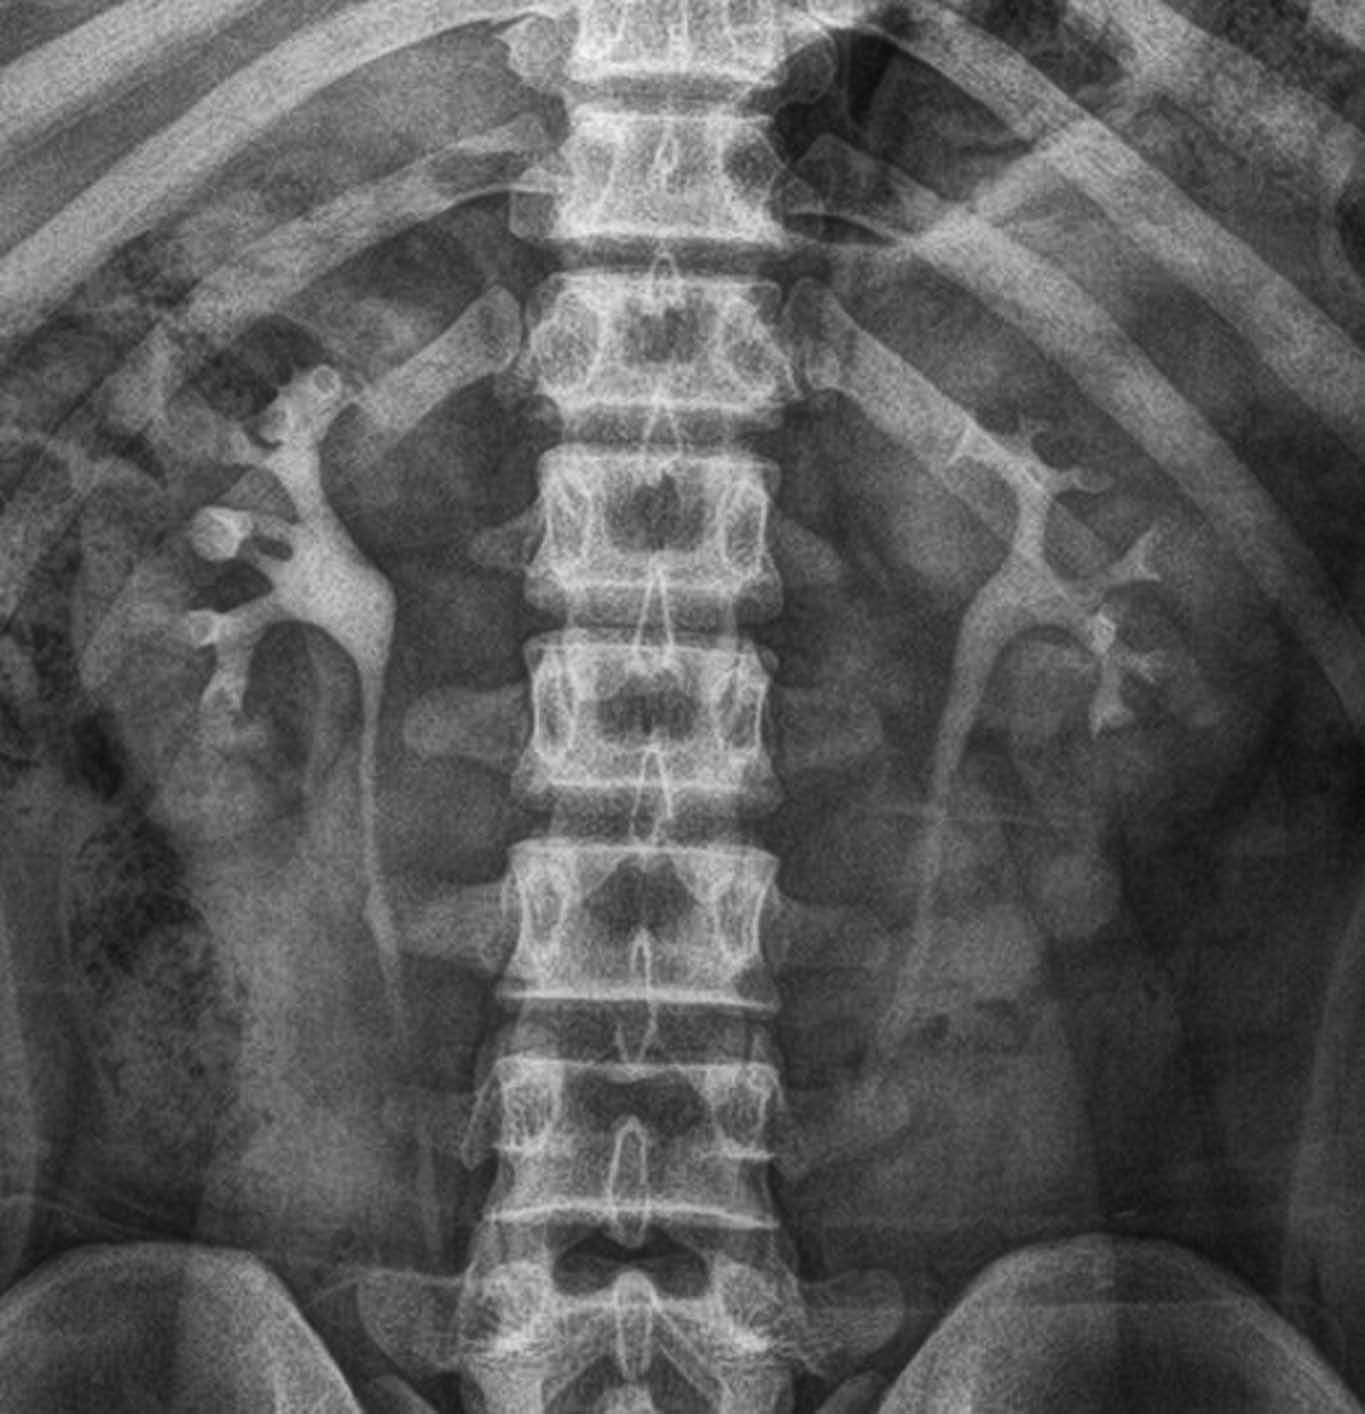
\includegraphics{./images/Image00329.jpg}
    \captionsetup{justification=centering}
    \caption{中间型肾盂,典型肾盂}
    \label{fig6-1-1}
\end{figure}

肾脏分肾实质及肾盂两部分。肾实质又分为皮质和髓质。肾脏皮质大多在肾脏表层,以两极为最厚,但也形成锥体间的分隔深入内部。肾的髓质在肾脏深部,有许多肾锥体构成,锥体的基底向外围,尖端向内形成乳头。乳头的顶部有7~50个乳头管开口,开口于肾小盏。肾盂上连大肾盏而下连输尿管。每一个大肾盏分底、颈及尖三部分,其底与肾盂相连,尖部则有1~2个小肾盏。每一个小肾盏又可分为体部及穹隆部,穹隆外缘内凹,为肾乳头伸入所致。通常有2~4个大肾盏,6~14个小肾盏,两侧可不对称。肾盂的容量通常为3~10ml。肾盂造影后表现为三种基本形态:①壶腹型肾盂:肾盂较大,肾盂与肾小盏直接相连,往往看不到肾大盏。②分支型肾盂:肾盂往往较小,相反肾大盏狭长、明显。③中间型肾盂:即所谓常见的典型肾盂,介于壶腹型与分支型之间。

依肾盂与肾窦的关系,肾盂又可分为:①肾内型肾盂:肾盂位于肾窦内,肾盏短小。②肾外型肾盂:肾盂位于肾窦外,肾盏则往往狭长。

肾盂的回流现象:在逆行尿路造影及部分静脉肾盂造影中,由于肾盂肾盏内压力增高,造影剂进入肾盂肾盏以外的区域,称为回流。回流有以下几种:

1.肾小管及肾质回流 造影剂自肾盂肾盏进入乳头小管并向收集系统扩散,表现为肾小盏向外呈刷状阴影,或进入肾小管旁肾皮质,呈扇形状影。

2.肾盏血管回流 即静脉周围回流,表现为肾盏附近有弓形或弧状的线条影。

3.肾盂淋巴管回流 表现为肾间质内有一条或多条线条状致密影。

4.肾盂、肾窦及肾盂、肾盏旁回流 造影剂自肾盏边缘外溢入肾窦或沿肾盏及肾旁组织到达输尿管周围。

二、输尿管

在尿路造影上输尿管为宽3~5mm,长25~30cm的细条状影,外形光滑,不时出现蠕动,有轻度弯曲或波浪状外形。

输尿管分段以骨性标记为界线,两髂嵴水平连线以上为上段,两骶髂关节下端水平连线与髂嵴水平连线之间为中段,以下为输尿管下段。输尿管有三个生理性狭窄部位,即输尿管与肾盂交界处、髂嵴水平处、输尿管与膀胱交界处。

三、膀胱

膀胱的形态、大小随其内充盈造影剂的量多少而改变,可为椭圆形、圆形等。密度均匀,边缘光滑。在静脉肾盂造影时,若输尿管下端有强烈蠕动,含造影剂的尿液成一条高密度的流注喷入膀胱内,叫输尿管喷射征(ureteral
jet sign)。

四、尿道

男性尿道分为前后两部分。后部自外向内可分为膜部和前列腺部,膜部尿道为最狭窄部,因其周围有外括约肌围绕。前部尿道较宽,自外向内为舟状窝、海绵体部与球部,球部尿道最宽。前尿道长13~17cm,后尿道长3~4cm,全尿道总长16~21cm。女性尿道很短,仅3.5cm。由膀胱颈部开始,向前下方开口于阴道口前壁。

\section{先天性异常}

\subsection{驼峰肾}

\begin{figure}
    \centering
    \subfloat[KUB片]{
        \begin{minipage}[b]{0.48\textwidth}
            \centering
            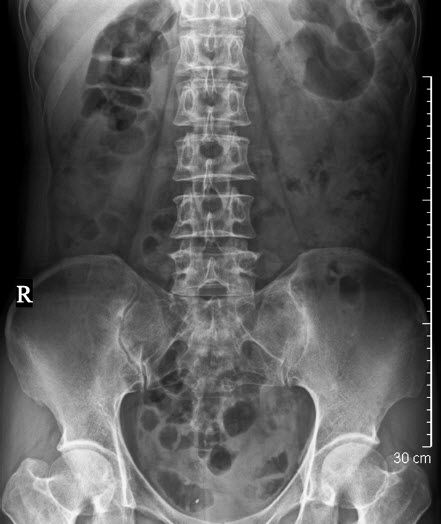
\includegraphics{./images/Image00330.jpg}
        \end{minipage}}
    \subfloat[IVP片]{
        \begin{minipage}[b]{0.48\textwidth}
            \centering
            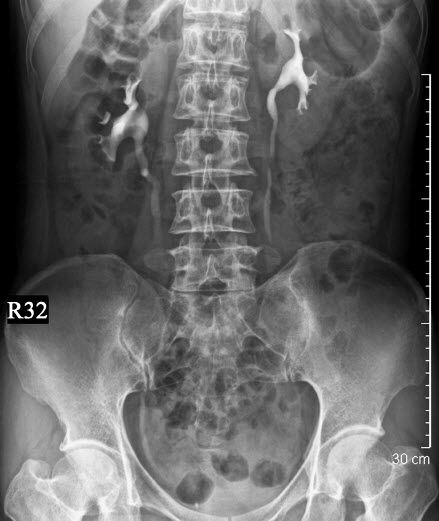
\includegraphics{./images/Image00331.jpg}
        \end{minipage}}\\
    \caption{}
    \label{fig6-2-1}
\end{figure}



\textbf{【病史摘要】}  女性,58岁。乏力、食欲不振、腰酸痛,伴有低热。

\textbf{【X线表现】}
KUB示:左侧肾脏外下缘局限性膨隆。造影后肾盂、肾盏显示清晰,未见明显受压及破坏改变。

\textbf{【X线诊断】}  左侧驼峰肾。

\textbf{【评  述】}
驼峰肾是一种肾脏形态正常的局部变形,多见于左肾,表现为肾脏局部外形的凸起,应与肾脏病变鉴别,动态增强CT及MRI上可见局部凸起为正常肾组织,皮髓质交界清晰。

\subsection{肾旋转异常}

\begin{figure}
    \centering
    \subfloat[KUB片]{
        \begin{minipage}[b]{0.48\textwidth}
            \centering
            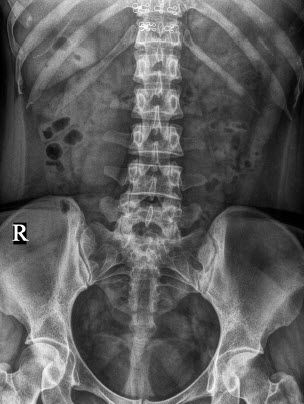
\includegraphics{./images/Image00332.jpg}
        \end{minipage}}
    \subfloat[IVP8分钟片]{
        \begin{minipage}[b]{0.48\textwidth}
            \centering
            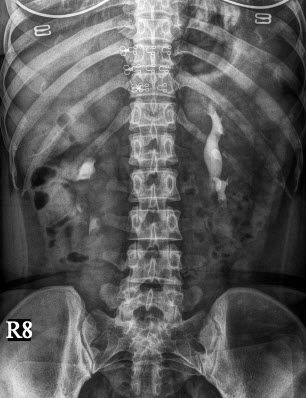
\includegraphics{./images/Image00333.jpg}
        \end{minipage}}\\
        \subfloat[IVP16分钟片]{
        \begin{minipage}[b]{0.48\textwidth}
            \centering
            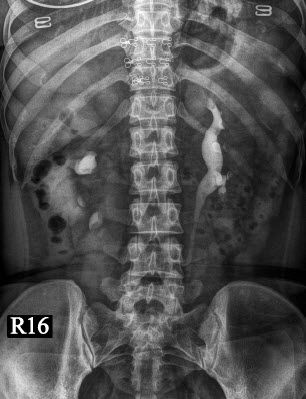
\includegraphics{./images/Image00334.jpg}
        \end{minipage}}
    \subfloat[IVP32分钟片]{
        \begin{minipage}[b]{0.48\textwidth}
            \centering
            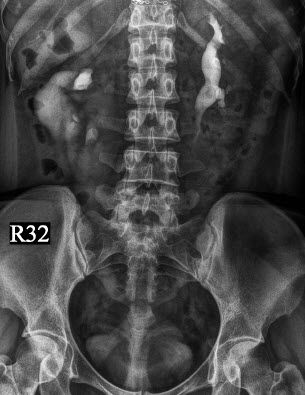
\includegraphics{./images/Image00335.jpg}
        \end{minipage}}\\
    \caption{}
    \label{fig6-2-2}
\end{figure}

\textbf{【病史摘要】}
女性,25岁。腰痛数年,近来加重,伴镜下血尿(+)。

\textbf{【X线表现】}
尿路造影示:右侧肾盂、肾盏方向异常,左侧肾盂扁平且伸长,肾长轴与中线交角变小,上1/3输尿管向外移位,双侧肾盂与输尿管交界处狭窄。

\textbf{【X线诊断】}  肾旋转不良。

\textbf{【评  述】}
胚胎发育过程中,肾脏从骨盆的始基处上升到最终的位置第2腰椎水平。在上升的过程中要经历一个沿肾脏本身纵轴向内90°的旋转,最后两肾门位置是直接朝内轻度偏前,两肾纵轴呈现八字形。在旋转过程中可以发生不旋转或旋转不足、旋转过度和反向旋转,这些称为旋转不良。肾旋转不良可以作为单独病变存在,也常可与融合肾、交叉肾合并存在。临床上肾旋转不良本身并不引起症状,但当输尿管因之而受压迫时,可导致输尿管梗阻并引起继发感染症状。尿路造影可以明确诊断。鉴别诊断主要是与融合肾,特别是与马蹄肾相区别,后者的位置较低,且一般为两侧性的旋转不良,在静脉肾盂造影片上可见两肾下极的肾皮质影互相连接,融合。

\subsection{异位肾}

\begin{figure}
    \centering
    \subfloat[KUB片]{
        \begin{minipage}[b]{0.48\textwidth}
            \centering
            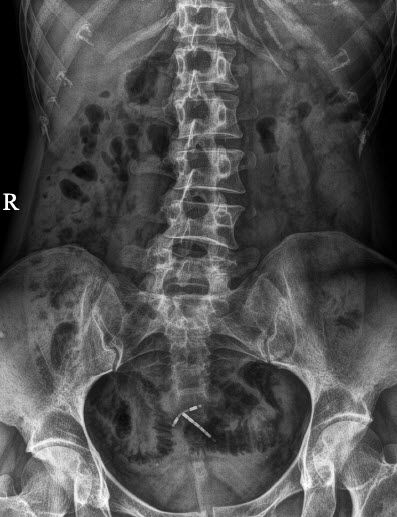
\includegraphics{./images/Image00336.jpg}
        \end{minipage}}
    \subfloat[IVP32分钟片]{
        \begin{minipage}[b]{0.48\textwidth}
            \centering
            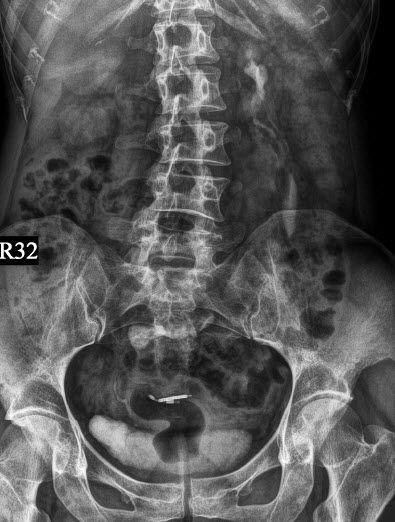
\includegraphics{./images/Image00337.jpg}
        \end{minipage}}\\
    \caption{}
    \label{fig6-2-3}
\end{figure}

\textbf{【病史摘要】}
女性,46岁。左腰酸痛,B超提示左肾积水,右肾未见。

\textbf{【X线表现】}
KUB平片;右肾区无肾影。尿路造影后示:骶骨前方见造影剂积聚,为异位缩小的右肾,左侧肾盂、肾盏扩张,左肾长轴与脊柱平行,左输尿管扩张,外移。

\textbf{【X线诊断】}  右侧盆腔异位肾,左肾旋转不良。

\textbf{【评  述】}
胚胎发育过程中,肾脏从骨盆的始基处上升到最终的位置第2腰椎水平。在此过程中因血供障碍或导向错误即形成异位肾。异位肾可以分为单纯性异位肾和交叉肾伴有融合或不伴融合两种。单纯性异位肾是指仅有上下位置改变而没有交叉到对侧肾脏。异位肾可以高于或低于正常肾的位置。低位最常见,常位于腰部、髂骨水平或骨盆腔区域。异位肾输尿管的长度没有迂曲延长,这是与肾下垂鉴别的重要特点。单纯性异位肾一般不发生症状,但易并发感染与结石。静脉肾盂造影可以明确诊断。

\subsection{肾发育不全}

\begin{figure}
    \centering
    \subfloat[KUB片]{
        \begin{minipage}[b]{0.48\textwidth}
            \centering
            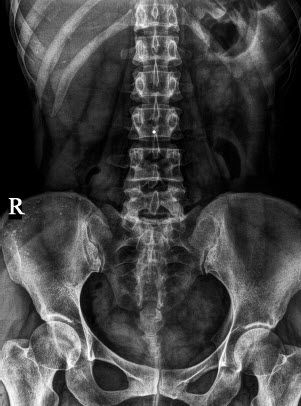
\includegraphics{./images/Image00338.jpg}
        \end{minipage}}
    \subfloat[IVP 16分钟片]{
        \begin{minipage}[b]{0.48\textwidth}
            \centering
            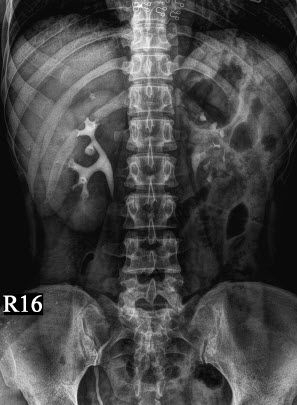
\includegraphics{./images/Image00339.jpg}
        \end{minipage}}\\
        \subfloat[IVP 32分钟片]{
        \begin{minipage}[b]{0.48\textwidth}
            \centering
            
\includegraphics{./images/Image00340.jpg}
        \end{minipage}}\\
    \caption{}
    \label{fig6-2-4}
\end{figure}



\textbf{【病史摘要】}
女性,42岁。进行性高血压,B超显示左侧肾脏体积缩小。

\textbf{【X线表现】}
尿路顺行造影检查时,可见左侧肾影明显缩小,肾实质菲薄,左侧肾盂、肾盏发育不良、狭小。左肾失去正常轮廓。右侧肾脏代偿性肥大。

\textbf{【X线诊断】}  左肾发育不全。

\textbf{【评  述】}
本病为肾脏在胚胎发育过程中生肾组织或后肾管发育障碍及血供不正常所致。肾脏因发育不全而体积变小,多为一侧性,两侧性罕见。发育不全的肾脏体积变小,肾功能变差。KUB平片及静脉肾盂造影可发现肾发育不全,但需与慢性肾盂肾炎及肾血管狭窄所致肾萎缩鉴别。

\subsection{马蹄肾}

\begin{figure}
    \centering
    \subfloat[KUB片]{
        \begin{minipage}[b]{0.48\textwidth}
            \centering
            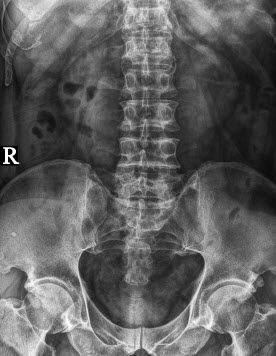
\includegraphics{./images/Image00341.jpg}
        \end{minipage}}
    \subfloat[IVP 16分钟片]{
        \begin{minipage}[b]{0.48\textwidth}
            \centering
            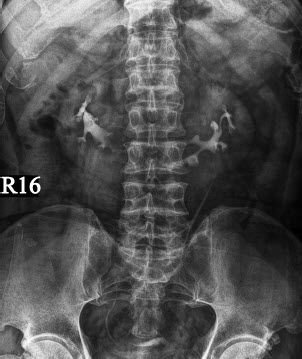
\includegraphics{./images/Image00342.jpg}
        \end{minipage}}\\
        \subfloat[IVP 32分钟片]{
        \begin{minipage}[b]{0.48\textwidth}
            \centering
            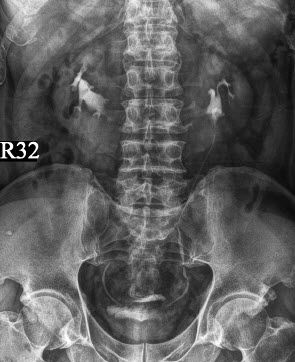
\includegraphics{./images/Image00343.jpg}
        \end{minipage}}\\
    \caption{}
    \label{fig6-2-5}
\end{figure}


\textbf{【病史摘要】}  男性,30岁。腰酸痛数月,尿检镜下血尿(++)。

\textbf{【X线表现】}
两侧肾影靠近脊椎,位置降低,长轴向外倾斜,下极向内靠近。尿路造影示下肾盏指向中线,肾盂、肾盏长轴上端向外下端向内呈倒八字形,输尿管向中线靠近。

\textbf{【X线诊断】}  马蹄肾。

\textbf{【评  述】}
马蹄肾发生于胚胎早期,是两侧肾脏胚基在两脐动脉之间被紧挤而融合的结果。融合大多在下极,发生在上极很少。两肾融合部分称为峡部,为肾实质或结缔组织所构成。两肾具有各自独立的肾盂和输尿管。马蹄肾多数是肾旋转不良,其长轴转为斜向内向下,使两肾的上极远离,两肾下极靠拢并联合于脊柱部位。肾盂因受融合影响,不能正常的旋转而位于前方,输尿管较正常为短。马蹄肾可无症状,亦可发生腰痛、血尿、排尿困难、腹部肿块等征状。常并发积水、结石、肾炎等,其血液供应比较复杂,可由肾动脉、髂总动脉、肠系膜下动脉供应。平片及静脉肾盂造影可确诊本病,但本病需与游走肾与异位肾鉴别。

\subsection{孤立肾}

\begin{figure}
    \centering
    \subfloat[KUB片]{
        \begin{minipage}[b]{0.48\textwidth}
            \centering
            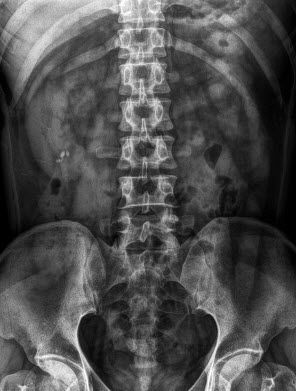
\includegraphics{./images/Image00344.jpg}
        \end{minipage}}
    \subfloat[IVP 32分钟片]{
        \begin{minipage}[b]{0.48\textwidth}
            \centering
            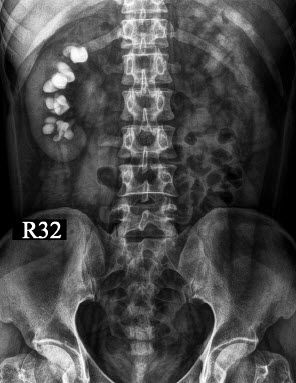
\includegraphics{./images/Image00345.jpg}
        \end{minipage}}\\
        \subfloat[IVP60分钟片]{
        \begin{minipage}[b]{0.7\textwidth}
            \centering
            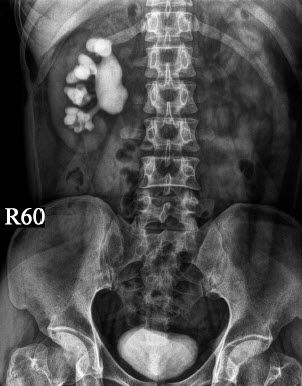
\includegraphics{./images/Image00346.jpg}
        \end{minipage}}\\
    \caption{}
    \label{fig6-2-6}
\end{figure}


\textbf{【病史摘要】}
男性,37岁。右腰部胀痛,有时有绞痛,B超示右肾结石,右肾积水。

\textbf{【X线表现】}
KUB示:右肾影增大明显,左肾区空虚,右肾下极见数枚小高密度结石影。尿路造影示右肾盂、肾盏扩张积水,左肾未显影。

\textbf{【X线诊断】}  右肾孤立肾,右肾结石,积水。

\textbf{【评  述】}
单侧肾缺如即孤立肾是一种相对常见的先天性发育异常。由于一侧生肾组织及输尿管芽不发育或仅有残缺的后肾组织所引起。故单侧肾缺如的同侧输尿管和膀胱三角区也同时缺如。平片及静脉肾盂造影可发现一侧肾区无肾影。需与异位肾及由于结核或炎症等病变所致肾无功能、萎缩鉴别。往往单靠静脉肾盂造影明确诊断有一定困难,CT或MRI可明确诊断。

\subsection{重复肾盂及重复输尿管}

\begin{figure}
    \centering
    \subfloat[KUB片]{
        \begin{minipage}[b]{0.48\textwidth}
            \centering
            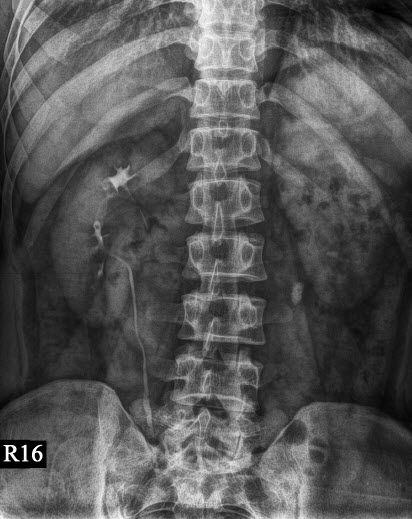
\includegraphics{./images/Image00347.jpg}
        \end{minipage}}
    \subfloat[IVP 32分钟片]{
        \begin{minipage}[b]{0.48\textwidth}
            \centering
            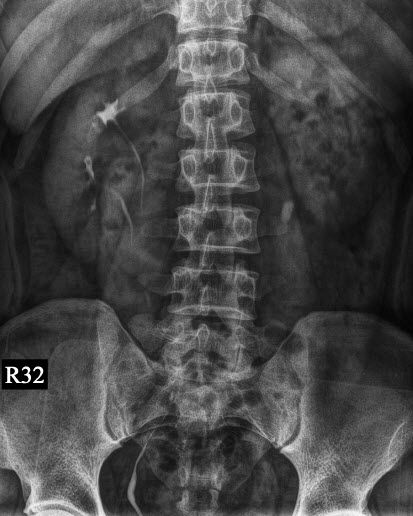
\includegraphics{./images/Image00348.jpg}
        \end{minipage}}\\
    \caption{}
    \label{fig6-2-7}
\end{figure}

\textbf{【病史摘要】}  女性,30岁。左肾绞痛入院,B超示左输尿管结石。

\textbf{【X线表现】}
尿路造影示:左输尿管上段结石,左肾积水,右侧双肾盂双输尿管重复畸形。

\textbf{【X线诊断】}
左输尿管上段结石伴左肾积水,右侧双肾盂双输尿管重复畸形。

\textbf{【评  述】}
重复肾盂及重复输尿管是上泌尿道最常见的先天畸形,在人群中的发病率为0.7%\textbf{~}
4%,一般发生于女性较多。重复畸形可分为部分性,形成一个单输尿管开口;亦可为完全性,两个输尿管开口于膀胱三角区。完全重复的输尿管系由中肾管两个输尿管芽形成,重复的输尿管完全分开,分别引流重复肾的两个肾盂的尿液,但此两个肾脏常融合成一体,称为双肾或重复肾。重复肾的上肾段发育较小,且常为单个肾盏,易于感染或积水。重复的输尿管分开,可并行或交叉向下引流,其进入膀胱依照Weigert-Meyer规律,即来自下肾盂的输尿管在进入膀胱时,越过来自上肾盂的输尿管,在膀胱内前者开口于后者的外上方,即上肾盂输尿管在膀胱开口位于下肾盂输尿管的内下方。重复输尿管往往伴有输尿管开口异位,男性开口可位于后尿道、精囊、输精管等处,女性可开口于尿道、阴道、外阴前庭等处,因异位开口于括约肌外,故常伴有尿失禁。静脉肾盂造影为本病的主要诊断方法。MR水成像技术,可显示静脉肾盂造影无显影的输尿管影,可作为补充诊断。

\subsection{先天性巨输尿管症}

\begin{figure}
    \centering
    \subfloat[KUB片]{
        \begin{minipage}[b]{0.48\textwidth}
            \centering
            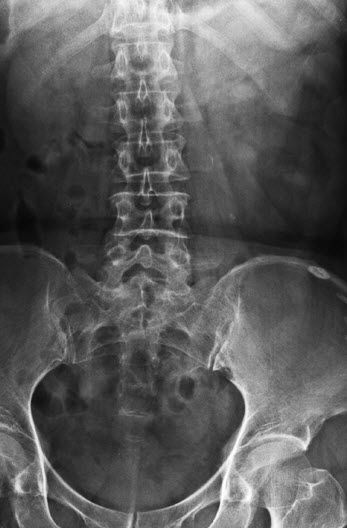
\includegraphics[height=.5\textheight]{./images/Image00349.jpg}
        \end{minipage}}
        \subfloat[IVP 60分钟片]{
        \begin{minipage}[b]{0.48\textwidth}
            \centering
            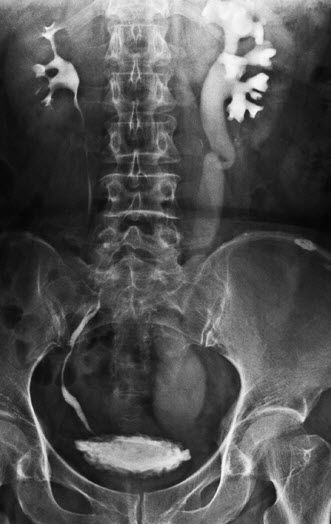
\includegraphics[height=.5\textheight]{./images/Image00350.jpg}
        \end{minipage}}\\
    \caption{}
    \label{fig6-2-8}
\end{figure}

\textbf{【病史摘要】}
女性,60岁。左侧腰部胀痛数月,B超示左输尿管扩张明显,左肾积水。

\textbf{【X线表现】}
尿路顺行造影示:左侧肾盂、肾盏扩张,左侧输尿管全程扩张,显影延迟。

\textbf{【X线诊断】}  左侧先天性巨输尿管。

\textbf{【评  述】}
先天性巨输尿管系一种先天性输尿管扩大,无输尿管膀胱出口以下的机械性梗阻及逆流。先天性巨输尿管主要是因为与膀胱毗邻的末端输尿管存在功能性狭窄,在X线上表现为近膀胱处输尿管常有短段状持续狭窄,为1\textbf{~}
2cm。本病诊断主要以尿路造影为主。MRI水成像亦有很大帮助,本病须与输尿管狭窄引起的输尿管扩张鉴别。前者狭窄及位置恒定为近膀胱处,以上输尿管扩张明显,程度较重。

\subsection{输尿管瓣膜症}

\begin{figure}
    \centering
    \subfloat[KUB片]{
        \begin{minipage}[b]{0.48\textwidth}
            \centering
            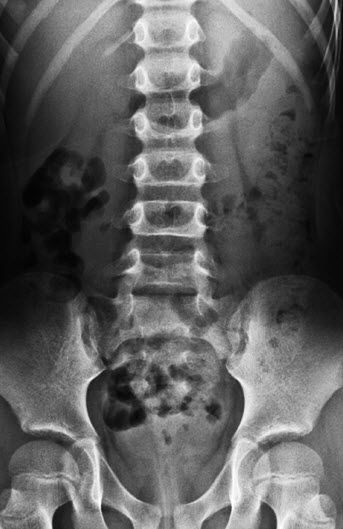
\includegraphics[height=.5\textheight]{./images/Image00351.jpg}
        \end{minipage}}
        \subfloat[IVP 32分钟片]{
        \begin{minipage}[b]{0.48\textwidth}
            \centering
            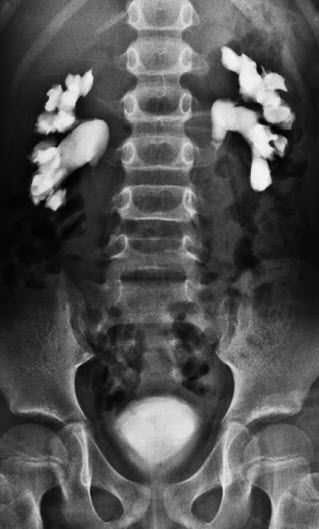
\includegraphics[height=.5\textheight]{./images/Image00352.jpg}
        \end{minipage}}\\
    \caption{}
    \label{fig6-2-9}
\end{figure}


\textbf{【病史摘要】}  男性,3岁。恶心、呕吐数天,腹部触及囊性包块。

\textbf{【X线表现】}
IVP示:双侧肾盂、肾盏扩张明显,双侧输尿管上端与肾盂连接处可见充盈缺损,以下输尿管未显影,膀胱显影正常。

\textbf{【X线诊断】}  双侧先天性输尿管瓣膜症。

\textbf{【评  述】}
先天性输尿管瓣膜症是罕见的病变。输尿管瓣膜是输尿管内一横行的皱襞,伴有平滑肌组织。该病发病机制不明。输尿管瓣膜症在病理上可分为两大类:①叶瓣型:可为单瓣、重瓣、多瓣。②环瓣型:环绕输尿管内壁生长,瓣膜表面可因炎症、肌层增生肥厚而增加了输尿管的狭窄与梗阻程度。尿路造影上表现为V形或倒V形充盈缺损。如瓣膜基底增生而较厚,充盈缺损可不规则。静脉肾盂造影是诊断输尿管瓣膜病变的主要手段。CT及MRI提供输尿管梗阻部位,而无法显示瓣膜的形状。输尿管的局部痉挛亦可以有局部狭窄的表现,但并不固定,其上段尿路大多无扩张积水现象,可与本病鉴别。

\subsection{腔静脉后输尿管}

\begin{figure}
    \centering
    \subfloat[]{
        \begin{minipage}[b]{0.48\textwidth}
            \centering
            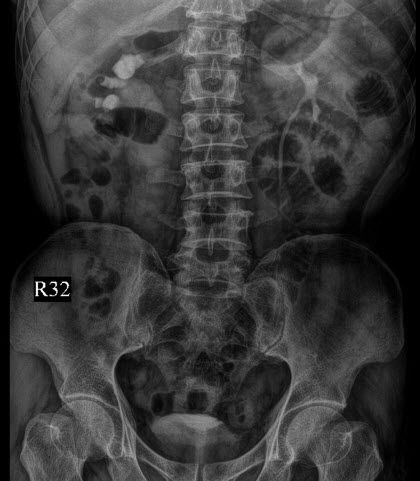
\includegraphics{./images/Image00353.jpg}
        \end{minipage}}
    \subfloat[]{
        \begin{minipage}[b]{0.48\textwidth}
            \centering
            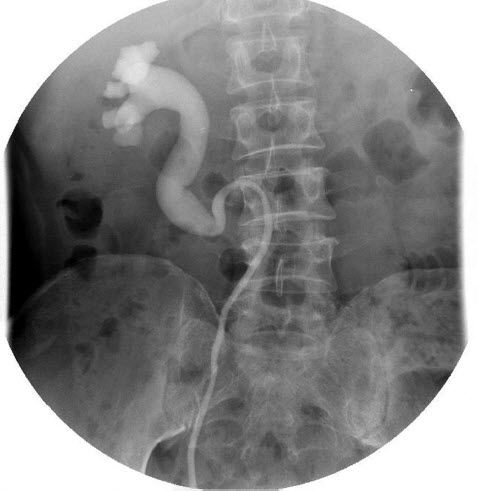
\includegraphics{./images/Image00354.jpg}
        \end{minipage}}\\
    \caption{}
    \label{fig6-2-10}
\end{figure}

\textbf{【病史摘要】}  男性,49岁。右侧腰部胀痛,B超示右肾积水。

\textbf{【X线表现】}
静脉肾盂造影示右肾积水,右输尿管上段扩张。逆行造影示右输尿管受压迂曲,右侧输尿管向中线移位,部分位于脊柱前。

\textbf{【X线诊断】}  右侧腔静脉后输尿管。

\textbf{【评  述】}
腔静脉后输尿管是一种少见的畸形,正常的输尿管走形位于下腔静脉的外侧。腔静脉后输尿管则从下腔静脉后绕至其内侧,再回到正常路线下行。病理上系腔静脉在胚胎发育过程中发生异常所致。病变多发生于右侧输尿管,静脉肾盂造影及逆行造影时,可见输尿管向中线移位,而与脊柱相重叠,上部扩大积水,输尿管形态呈镰刀状或S样畸形。侧位片见输尿管被推压而紧贴在第3\textbf{~}
4腰椎体的前缘。本病诊断主要为静脉肾盂造影及逆行造影,典型表现可以诊断。但需排除后腹膜占位引起的输尿管移位,CT扫描有助于进一步明确诊断。

\subsection{先天性输尿管狭窄}

\begin{figure}
    \centering
    \subfloat[KUB片]{
        \begin{minipage}[b]{0.48\textwidth}
            \centering
            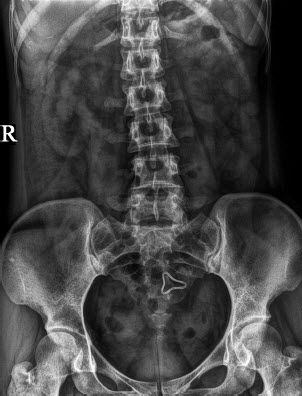
\includegraphics{./images/Image00355.jpg}
        \end{minipage}}
    \subfloat[IVP 16分钟片]{
        \begin{minipage}[b]{0.48\textwidth}
            \centering
            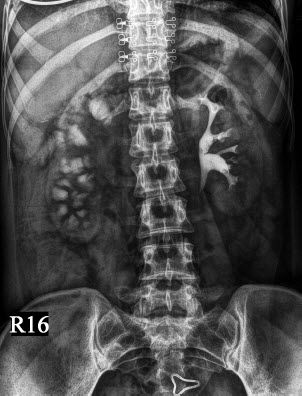
\includegraphics{./images/Image00356.jpg}
        \end{minipage}}\\
        \subfloat[IVP 32分钟片]{
        \begin{minipage}[b]{0.5\textwidth}
            \centering
            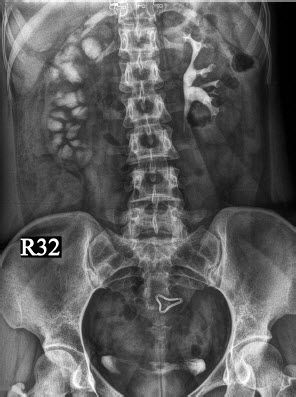
\includegraphics{./images/Image00357.jpg}
        \end{minipage}}
    \subfloat[右侧RP造影片]{
        \begin{minipage}[b]{0.5\textwidth}
            \centering
            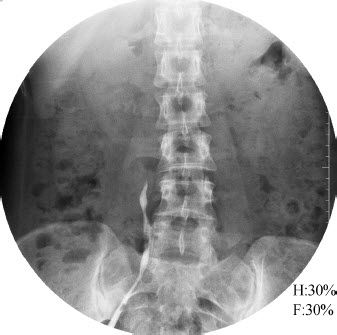
\includegraphics{./images/Image00358.jpg}
        \end{minipage}}\\
    \caption{}
    \label{fig6-2-11}
\end{figure}


\textbf{【病史摘要】}  女性,28岁。体检时B超发现右肾积水。

\textbf{【X线表现】}
尿路顺行造影示:右肾盏扩张,右输尿管未显影。后做逆行尿路造影,示导管插入至L3椎体右侧横突下缘水平,经导管注入造影剂示以上输尿管未显影。

\textbf{【X线诊断】}  右输尿管上段狭窄,右肾积水。

\textbf{【评  述】}
本病原因不明。病理上可以为输尿管粘膜过长,因粘膜的聚集而发生功能性狭窄,也可以为外鞘膜分离导致粘膜皱襞纵行伸直而产生器质性狭窄。狭窄部位常见于肾盂输尿管交界处和输尿管膀胱连接处,中段极少见。1963年Compbell报道19046例小儿尸解中共有123例先天性输尿管狭窄,发生率为0.6%。临床上常由于肾盂积水产生腹部包块而就诊,同时可有腹痛、合并泌尿系感染等。本病需与迷走血管压迫输尿管鉴别,选择性血管造影可见迷走血管压迫的情况。本病主要依靠静脉肾盂造影确诊,MRU对肾功能不好的患者有很大的帮助。

\subsection{膀胱憩室}

\begin{figure}
    \centering
    \subfloat[KUB片]{
        \begin{minipage}[b]{0.48\textwidth}
            \centering
            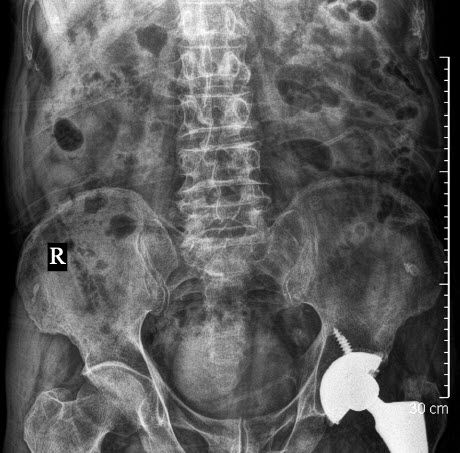
\includegraphics[height=.5\textheight]{./images/Image00359.jpg}
        \end{minipage}}
    \subfloat[IVP32分钟片]{
        \begin{minipage}[b]{0.48\textwidth}
            \centering
            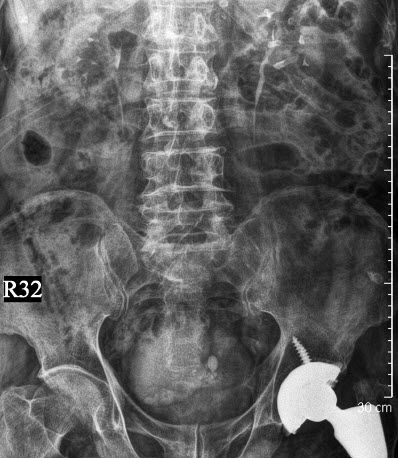
\includegraphics[height=.5\textheight]{./images/Image00360.jpg}
        \end{minipage}}\\
    \caption{}
    \label{fig6-2-12}
\end{figure}

\textbf{【病史摘要】}  男性,86岁。尿频,尿急,淋漓不尽。

\textbf{【X线表现】}
尿路造影后示:膀胱区见类圆形高密度影,平片无此现象,考虑膀胱憩室、造影剂充填。

\textbf{【X线诊断】}  膀胱憩室。

\textbf{【评  述】}
膀胱憩室可能为膀胱壁内胚胎组织发育而成。特别是在胚胎期与中肾管或尿囊连接处发生,或可由于输尿管芽的多发,以及脐尿管的残余等先天原因构成。大多由于膀胱壁内肌层存在薄弱点,和与梗阻有关的膀胱内压的增加而形成。好发于膀胱侧后部,常见于三角区上方,成袋形向外突出,颈部较小,开口区与输尿管接近。膀胱排空后,隔数秒钟,又有少数尿液排出,为较特征性症状。憩室内可继发结石亦可发生肿瘤。静脉肾盂造影或膀胱造影可确诊。本病需与输尿管远端囊样扩张鉴别,静脉肾盂造影有明显优势。

\section{泌尿系结石}

\subsection{肾铸形结石}

\textbf{【病史摘要】}
女性,47岁。右腰部胀痛数月,近来加重,B超示右肾结石。

\begin{figure}[H]
    \centering
    \subfloat[KUB片]{
        \begin{minipage}[b]{0.48\textwidth}
            \centering
            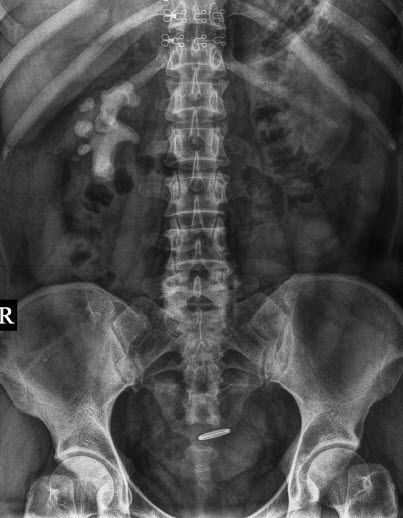
\includegraphics{./images/Image00361.jpg}
        \end{minipage}}
    \subfloat[IVP32分钟片]{
        \begin{minipage}[b]{0.48\textwidth}
            \centering
            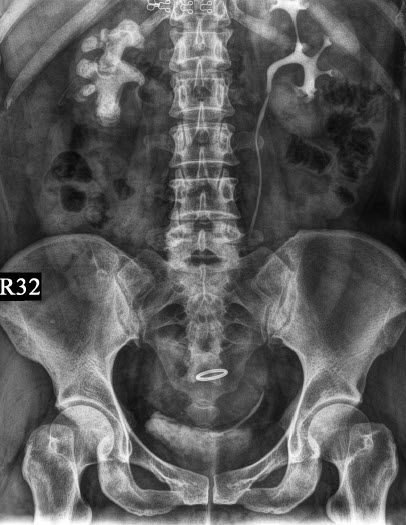
\includegraphics{./images/Image00362.jpg}
        \end{minipage}}\\
    \caption{}
    \label{fig6-3-1}
\end{figure}

\textbf{【X线表现】}
平片示:右肾区见异常高密度影,呈鹿角形。尿路造影示肾盂、肾盏显影。

\textbf{【X线诊断】}  右肾铸形结石。

\textbf{【评  述】}
肾结石占据整个肾盂、肾盏称铸形结石或塑形结石、鹿角形结石,也称珊瑚状结石。尿石症为泌尿系统最常见疾病之一。结石的形成机制复杂且无确切定论,主要有如下学说:①晶体沉淀学说。②基质核心学说。③抑制剂缺乏学说。④酸碱度改变学说。⑤激素学说。

泌尿系结石常为两种或两种以上且以一种晶体为主混合而成。在我国,最常见为磷酸钙和草酸钙为主的混合结石。90%以上结石为吸收X线的盐类,平片可以看出。肾铸形结石占据整个肾盂、肾盏,直接影响肾分泌功能,直至功能完全丧失。肾结石的鉴别诊断主要与肾结核钙化区别,肾结核钙化多偏近肾的边缘,即在肾皮质内,不能移动,此外可见相应的肾盏边缘常有破坏。与肿瘤内钙化的区别是后者有局部的肾外形扩大,肾盂、肾盏有压迫或浸润现象。

\subsection{肾盂和肾盏结石}

\begin{figure}
    \centering
    \subfloat[KUB片]{
        \begin{minipage}[b]{0.48\textwidth}
            \centering
            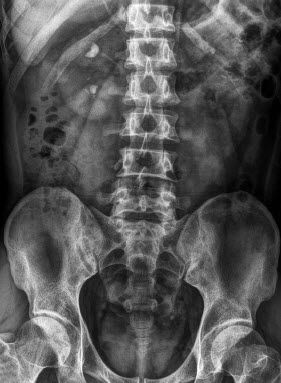
\includegraphics{./images/Image00363.jpg}
        \end{minipage}}
    \subfloat[IVP16分钟片]{
        \begin{minipage}[b]{0.48\textwidth}
            \centering
            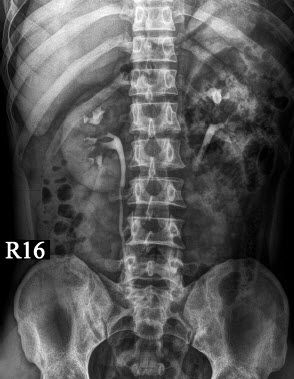
\includegraphics{./images/Image00364.jpg}
        \end{minipage}}\\
    \subfloat[IVP32分钟片]{
        \begin{minipage}[b]{0.48\textwidth}
            \centering
            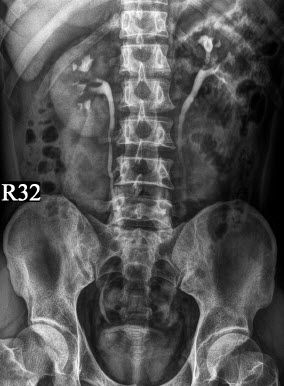
\includegraphics{./images/Image00365.jpg}
        \end{minipage}}\\
    \caption{}
    \label{fig6-3-2}
\end{figure}



\textbf{【病史摘要】}  男性,35岁。左腰部痛1天。

\textbf{【X线表现】}
双侧肾区见不规则高密度影,左输尿管下段见小高密度影,静脉肾盂造影示右肾区高密度影位于肾上盏与肾下盏内,左输尿管上段略扩张。

\textbf{【X线诊断】}
右肾盏结石,左肾结石,左输尿管下段结石,左肾轻度积水。

\textbf{【评  述】}
肾盂结石呈圆形、类圆形或类肾盂形态的三角形,可致密、浅淡或分层。结石可引起肾盂、肾盏的损伤、感染和阻塞,导致上皮脱落、溃疡并最后有纤维瘢痕形成。结石引起的梗阻常是不完全性的,尿液可通过结石的周围而流入输尿管,肾盂或肾盏的壁可以肥厚并纤维化,因此很少发生扩大。若肾结石位于肾盂与输尿管交界处,则肾盂积水就明显,肾盏亦扩大。大多数结石KUB平片就能确诊。右上腹的结石应与胆囊结石鉴别,加摄侧位片,肾结石与脊柱重叠而胆囊结石位于脊柱前方。静脉肾盂造影可对肾功能进行初步评价。

\subsection{输尿管结石}

\begin{figure}
    \centering
    \subfloat[KUB片]{
        \begin{minipage}[b]{0.48\textwidth}
            \centering
            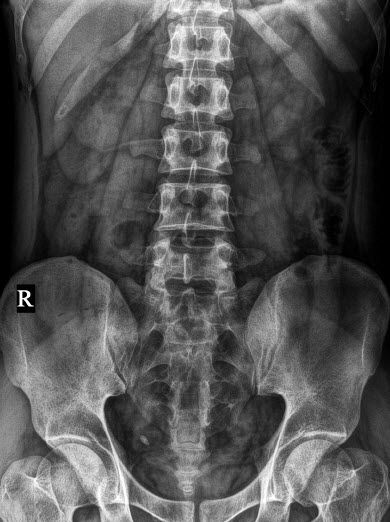
\includegraphics[height=.4\textheight]{./images/Image00366.jpg}
        \end{minipage}}
    \subfloat[IVP32分钟片]{
        \begin{minipage}[b]{0.48\textwidth}
            \centering
            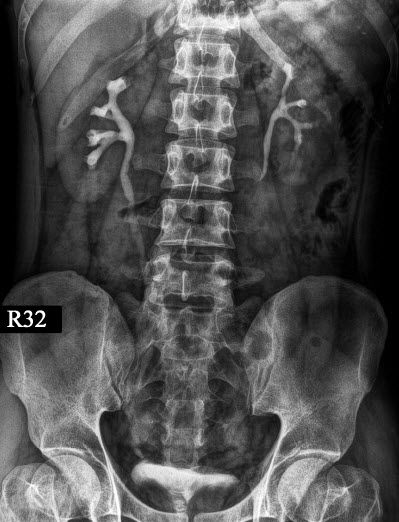
\includegraphics[height=.4\textheight]{./images/Image00367.jpg}
        \end{minipage}}\\
    \caption{}
    \label{fig6-3-3}
\end{figure}

\textbf{【病史摘要】}  男性,28岁。右侧腰部绞痛1天。

\textbf{【X线表现】}
膀胱区右侧见小高密度影,尿路造影示右肾盂、肾盏扩张,肾盏杯口消失,右输尿管全程扩张。

\textbf{【X线诊断】}  右输尿管末端结石伴右肾积水。

\textbf{【评  述】}
输尿管结石主要是由肾结石落入输尿管内形成。输尿管结石引起的病理改变主要为梗阻,可继发结石周围的输尿管炎和输尿管周围炎,晚期纤维组织增生,管壁增厚并发狭窄。感染引起的狭窄多位于结石以下。输尿管结石多位于输尿管解剖生理狭窄处,即输尿管与肾盂交界处,输尿管跨过髂动脉处,输尿管进入膀胱外肌层处以及输尿管在膀胱内的开口处。其中以输尿管跨过髂动脉处以及进入膀胱的两个部位最为常见。输尿管结石的诊断以KUB平片为主,结石位于输尿管行经区,形态多呈长圆形或梭形,其长轴与输尿管的长轴一致。腰椎的横突和骶髂骨可与结石影重叠,应摄斜位片鉴别。静脉肾盂造影可明确结石位置以及有无肾积水及肾功能情况。阴性结石及静脉肾盂造影不显影患者可行MRU及CT检查。鉴别诊断主要与肠道内容物及肠系膜淋巴结钙化的鉴别,后者位置常可变动且密度不均匀。与动脉壁钙化的区别是后者多呈线条状且多为平行的与盆腔静脉石的区别是后者位置较偏外,多为光滑圆形,大多边缘密度较浓,中心较淡,且往往是多发的。

\subsection{膀胱结石}

\begin{figure}[!htbp]
    \centering
    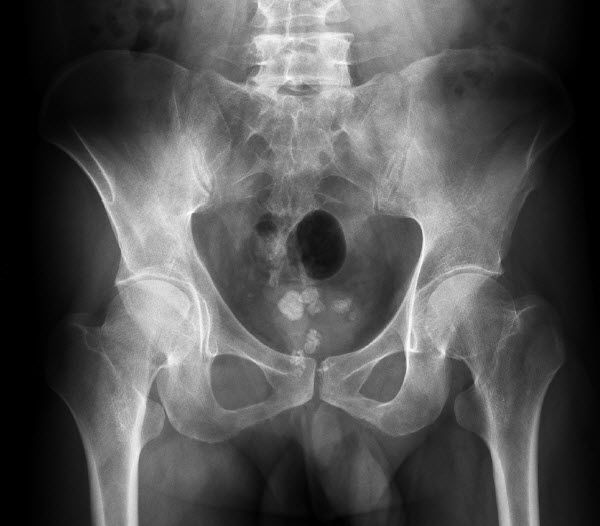
\includegraphics{./images/Image00368.jpg}
    \captionsetup{justification=centering}
    \caption{KUB片}
    \label{fig6-3-4}
\end{figure}

\textbf{【病史摘要】}  男性,38岁。尿不尽,尿痛,尿检镜下血尿(+++)。

\textbf{【X线表现】}  KUB平片示:膀胱区多发大小不等高密度影。

\textbf{【X线诊断】}  膀胱结石。

\textbf{【评  述】}
本病大多见于男性,约占95%。可发生于任何年龄,以50岁以上的老年人较常见。膀胱结石大多是由上尿路结石坠入膀胱内逐渐变大的,形态大小多样,小如沙砾,大者能占据整个膀胱。膀胱结石主要依靠平片检查,膀胱结石形态多样,可单发或多发,可随体位变动。膀胱造影可证实平片发现的膀胱内结石。也可发现阴性结石及膀胱憩室内的结石。膀胱结石需与前列腺钙化、粪石、静脉石、盆腔肿瘤钙化鉴别。进一步确诊可行CT或B超检查。

\subsection{尿道结石}

\begin{figure}
    \centering
    \subfloat[膀胱区平片]{
        \begin{minipage}[b]{0.48\textwidth}
            \centering
            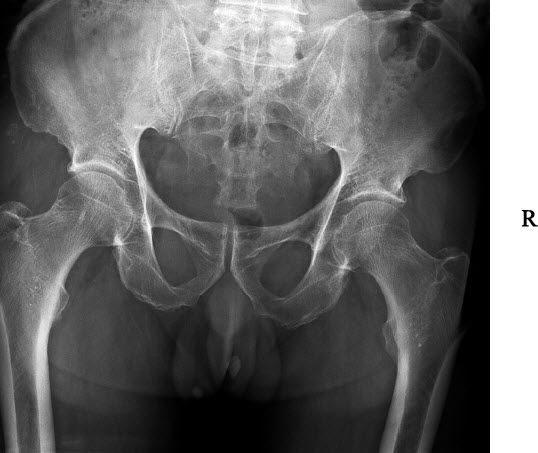
\includegraphics[height=.25\textheight]{./images/Image00369.jpg}
        \end{minipage}}
    \subfloat[尿道侧位片]{
        \begin{minipage}[b]{0.48\textwidth}
            \centering
            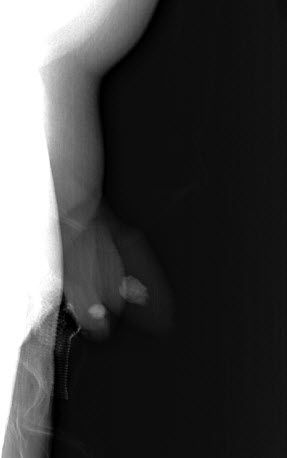
\includegraphics[height=.25\textheight]{./images/Image00370.jpg}
        \end{minipage}}\\
    \caption{}
    \label{fig6-3-5}
\end{figure}

\textbf{【病史摘要】}  男性,62岁。尿不尽,尿痛。

\textbf{【X线表现】}
尿道舟状窝见高密度影,边缘毛糙,右侧阴囊区见高密度影。

\textbf{【X线诊断】}  尿道结石。右侧阴囊区高密度影。

\textbf{【评  述】}
尿道结石较少见,占泌尿道结石的10%左右,多见于男性。尿道结石一般为单发,也可以为多发。一般结石较小,结石所在部位不同,形状也不同。结石常位于尿道,次之在球部和舟状窝内。临床上主要表现为会阴部或阴茎疼痛,尿频,尿急,尿流变慢而无力,慢性尿潴留,滴尿,尿失禁和血尿。扪诊时,有时可扪到结石。

X线平片能诊断,所见结石与尿道平行,结石一般较小。鉴别诊断一般与阴茎静脉石及慢性海绵体炎所致的钙化鉴别,但其引起的钙化位置及形态均不相同,较易鉴别。

\subsection{异物性膀胱结石}

\begin{figure}[!htbp]
    \centering
    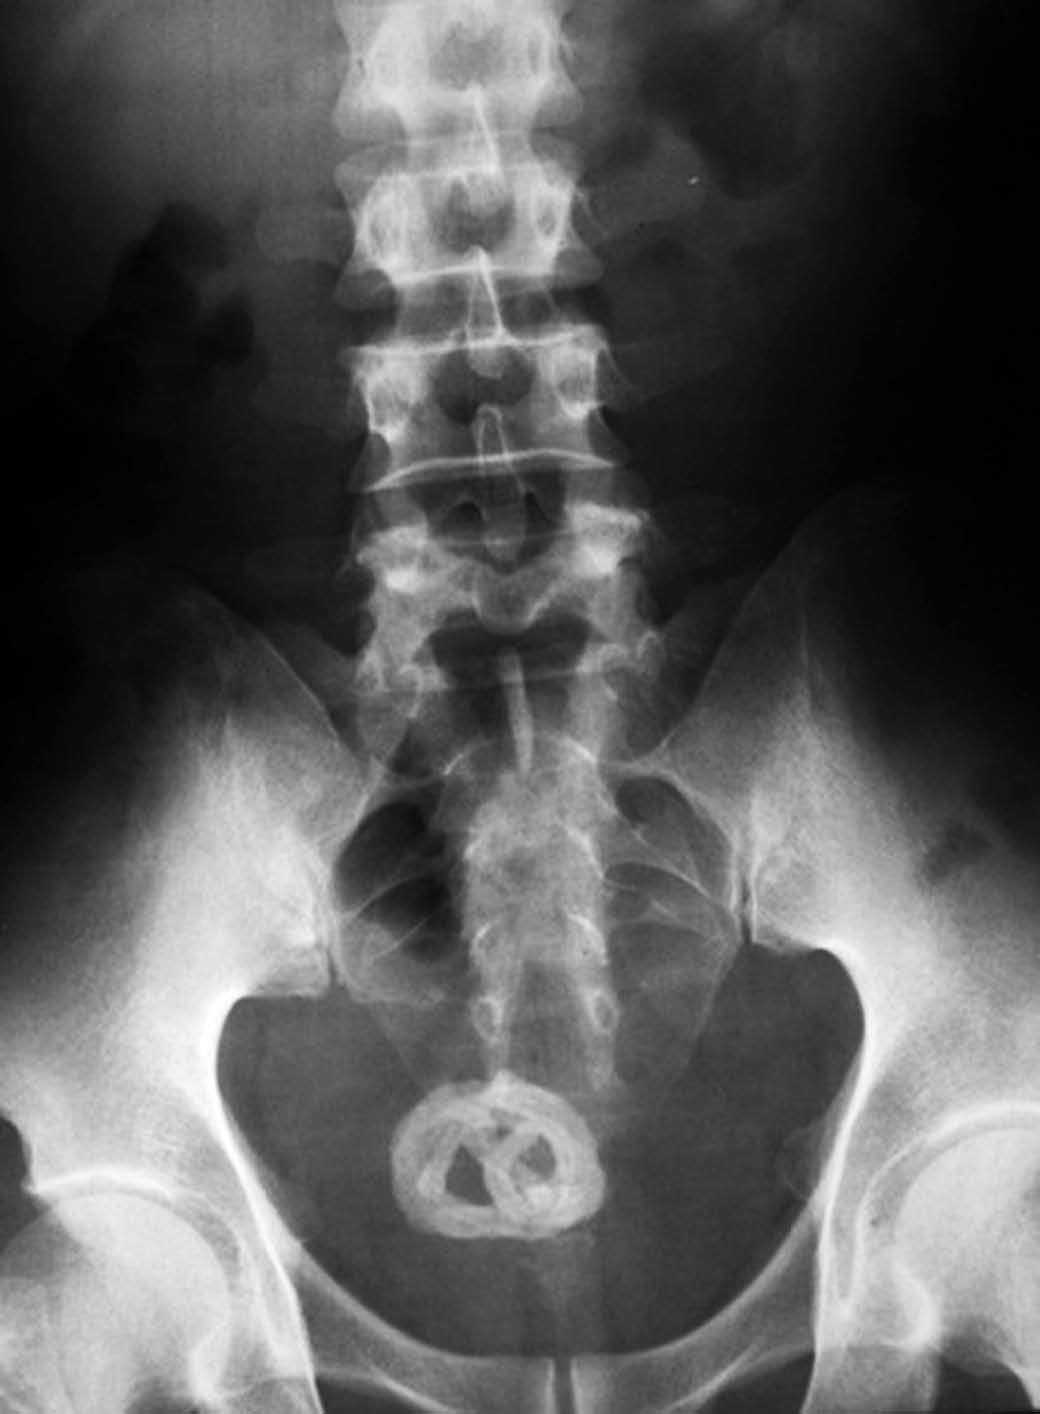
\includegraphics{./images/Image00371.jpg}
    \captionsetup{justification=centering}
    \caption{KUB平片}
    \label{fig6-3-6}
\end{figure}

\textbf{【病史摘要】}  男性,25岁。有异物插入尿道史,现尿频、尿急。

\textbf{【X线表现】}  膀胱区见蜷曲的条形高密度影。

\textbf{【X线诊断】}  异物性膀胱结石。

\textbf{【评  述】}
异物性膀胱结石少见,异物存留在膀胱中,形成以异物为核心的结石,结石可逐渐增大,异物性膀胱结石一般与在膀胱中的异物形态相一致。异物最多见于从尿道口插入,其次为手术遗留。结合病史,可明确诊断。

\section{泌尿系结核和非特异性炎症}

\subsection{结核性肾皮质脓疡}

\begin{figure}[!htbp]
    \centering
    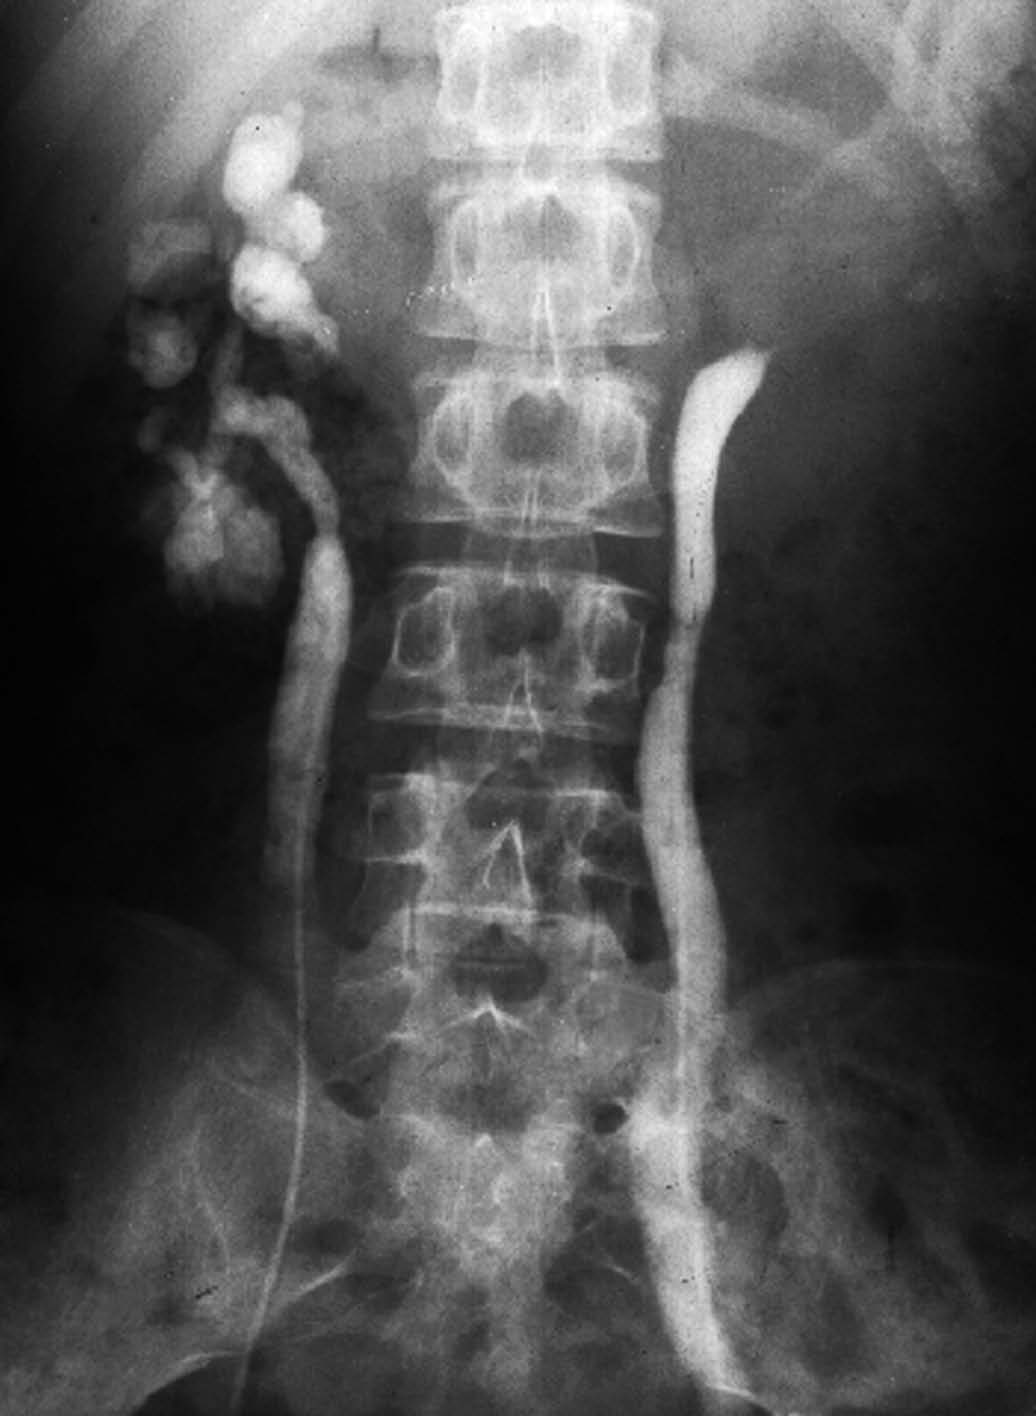
\includegraphics{./images/Image00372.jpg}
    \captionsetup{justification=centering}
    \caption{IVP32分钟平片}
    \label{fig6-4-1}
\end{figure}

\textbf{【病史摘要】}
男性,35岁。右侧腰痛半年余,伴有低热、盗汗、尿频、尿痛,有脓尿1个月余。

\textbf{【X线表现】}
逆行造影示:右侧肾盂、肾盏变形,肾盏与肾实质内脓腔连通形成大而不规则的脓腔,输尿管近端也受累。同侧腰大肌影消失。左侧输尿管全程扩张,左肾未显影。

\textbf{【X线诊断】}
右肾及双侧输尿管结核伴右肾皮质脓疡形成,左肾未显影。

\textbf{【评  述】}
结核是常见的泌尿系统疾病,肾、输尿管、膀胱均可累及,其中尤以肾结核最为重要。肾是泌尿系及男性生殖系统结核病的初发器官,而肾结核多继发于身体其他器官的结核病灶。肺结核患者中,1%\textbf{~}
4%的患者有临床泌尿生殖系统结核病。骨关节结核患者中,尿结核杆菌阳性占20%。结核杆菌到达肾的路径有四种,经血液、尿路、淋巴管和直接蔓延。结核杆菌经血液到达肾是最重要的途径。结核杆菌血行到达肾脏,即原发病变在肾小球的血管丛,病变的特点是位于肾皮质部分,多发,两侧性,病变多数可以自愈,仅少数随后发展为慢性进行性结核病变。

病变进展,皮质内的结核结节逐渐扩大互相融合,在中心发生坏死,病变侵入肾的髓质或是病灶破入肾曲小管,结核杆菌经肾曲小管到达肾乳头,在肾的髓质形成病灶。病灶进行性发展引起临床症状,这就是临床肾结核。临床肾结核阶段,肾乳头产生溃疡,直接侵犯相应肾盏粘膜和肌层,逐渐产生狭窄使相应锥体很快产生空洞,空洞壁为不规则的肉芽组织,表现为肾杯口的破坏和肾盏体、颈部僵硬狭窄,多个空洞形成。在病变的发展过程中,因机体免疫力强弱不同,病灶的反应也不相同。肾结核往往新老病灶同时存在,病变发展互相重叠,不能单独孤立分开,有的只是某一特征性表现在X线片显示明显而已。本病主要以静脉肾盂造影诊断为主,无肾功能者,可行MRU检查。CT可明确脓疡的存在和部位。结核性肾皮质脓肿需与灶性肾炎、化脓性脓肿和肾囊肿鉴别。需密切结合临床、检验,确诊为细菌学检查。影像学上结核性脓肾常伴有其他结核性改变如钙化,或纤维增生造成肾脏变形缩小。

\subsection{空洞溃疡型肾结核}

\begin{figure}[!htbp]
    \centering
    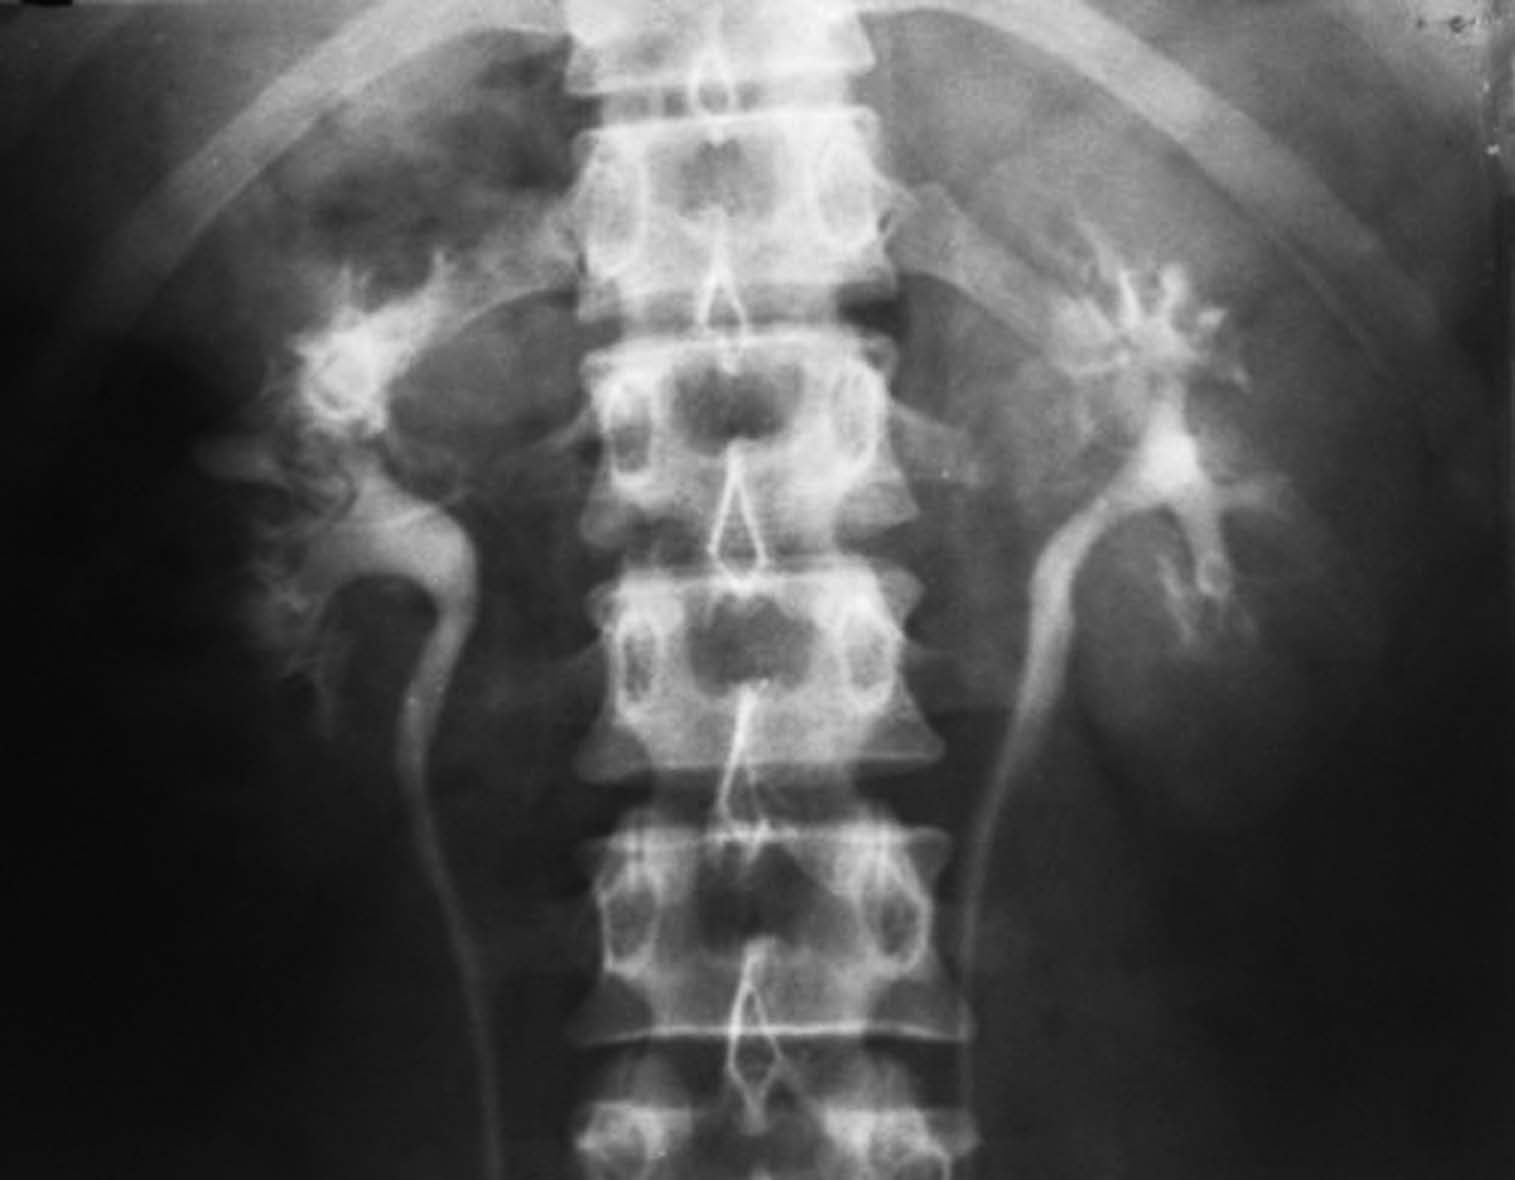
\includegraphics{./images/Image00373.jpg}
    \captionsetup{justification=centering}
    \caption{IVP平片}
    \label{fig6-4-2}
\end{figure}

\textbf{【病史摘要】}  男性,33岁。肺结核病史3年,现腰部酸痛,加重3天。

\textbf{【X线表现】}
尿路造影示:双侧肾盏杯口虫蚀样改变,边缘毛糙,可见空洞形成。

\textbf{【X线诊断】}  双肾结核。

\textbf{【评  述】}
此种类型常见。肾皮质脓疡继续发展,侵犯肾乳头,继而侵犯肾盏。肾小盏杯口部分显示有虫蚀样改变,边缘毛糙。破坏区扩大,由一个肾小盏扩大到数个小盏,干酪物质破溃形成空洞。造影显示为云朵状,边缘不整的空洞阴影和肾盂、肾盏虫蚀样改变。由于肉芽增生形成肾盏颈部瘢痕狭窄。逆行造影时,造影剂无法进入病变的肾盏而显示肾盏缺如。但静脉肾盂造影可显示出狭窄上方的肾盏,并见狭窄前扩张。

\subsection{结核脓肾和膀胱结核}

\begin{figure}
    \centering
    \subfloat[KUB平片]{
        \begin{minipage}[b]{0.48\textwidth}
            \centering
            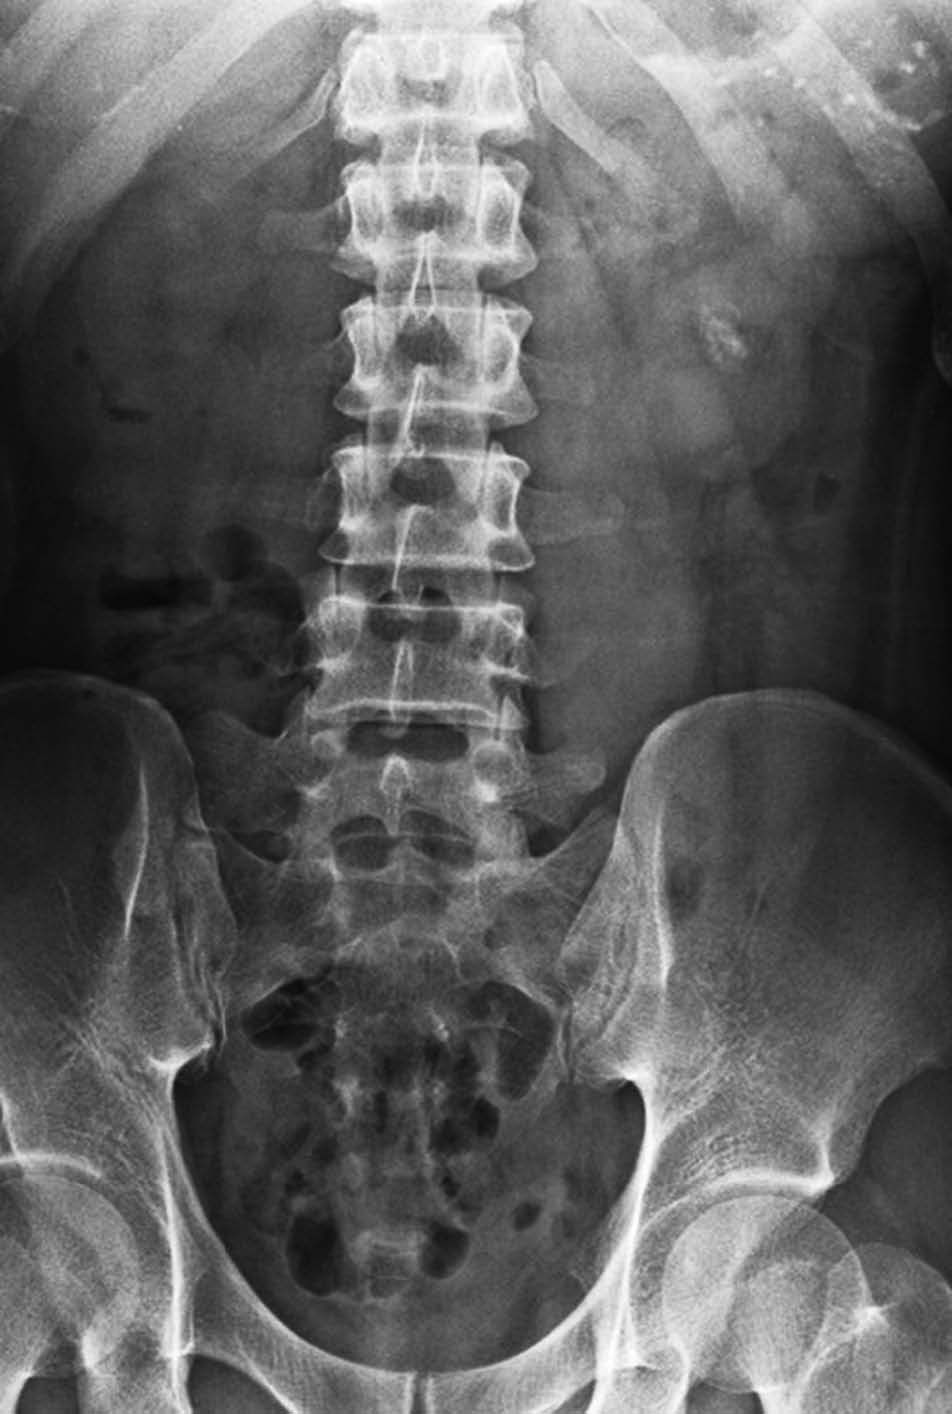
\includegraphics{./images/Image00374.jpg}
        \end{minipage}}
    \subfloat[IVP片]{
        \begin{minipage}[b]{0.48\textwidth}
            \centering
            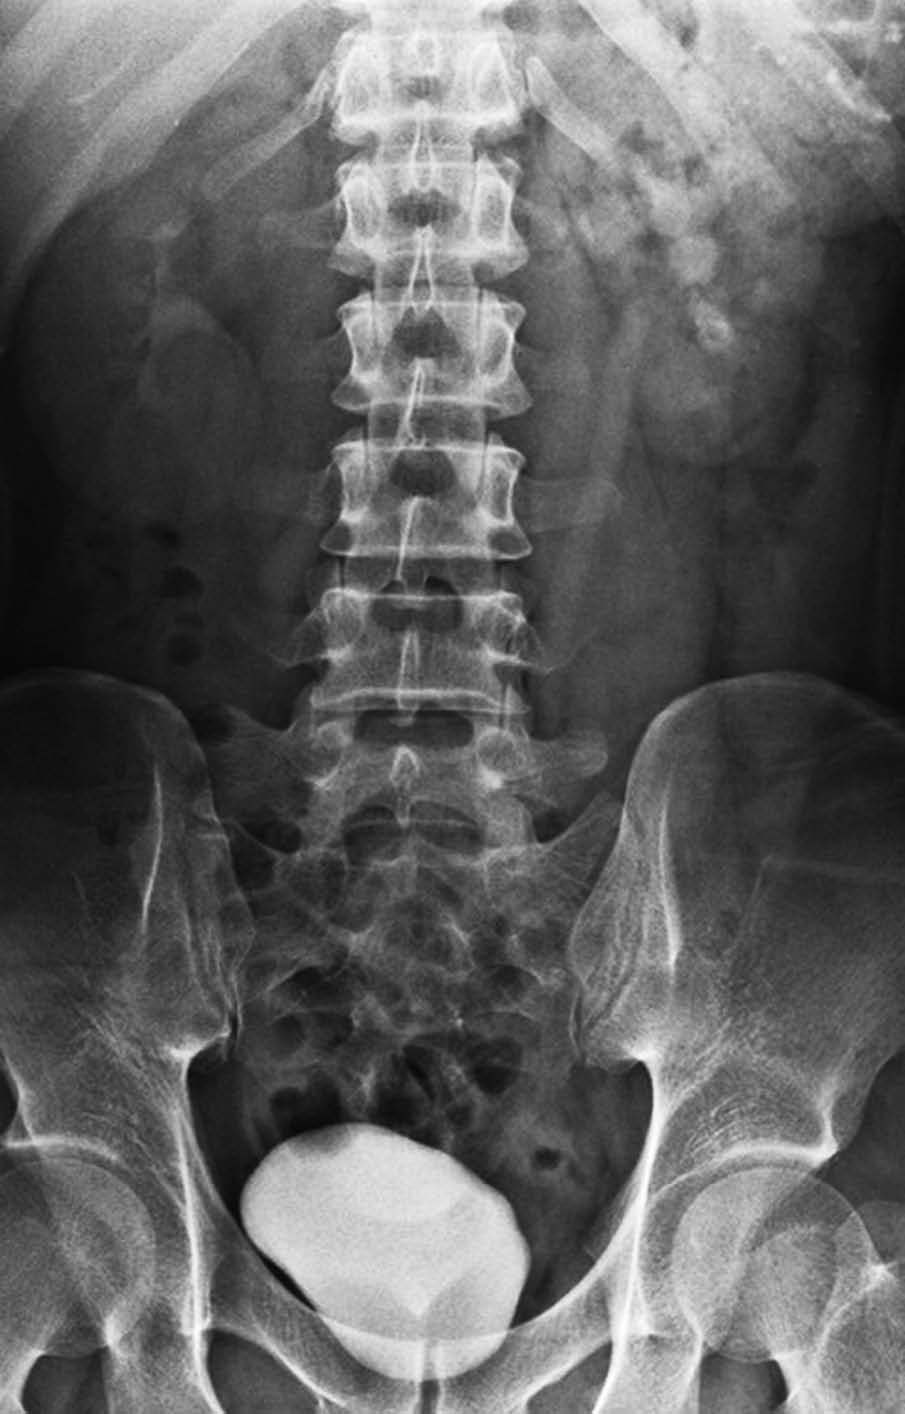
\includegraphics{./images/Image00375.jpg}
        \end{minipage}}\\
    \caption{}
    \label{fig6-4-3}
\end{figure}

\textbf{【病史摘要】}
男性,45岁。有肾结核病史2年,近来乏力,食欲不振。

\textbf{【X线表现】}
左肾局限性膨隆,左肾实质见钙化灶,尿路造影示左肾盏扩张积水,边缘毛糙,虫蚀样改变,左输尿管扩张。

\textbf{【X线诊断】}  左肾结核。

\textbf{【评  述】}
病变继续发展,使输尿管痉挛、狭窄、梗塞而形成肾盂积脓。肾脏轮廓扩大,肾盂扩张。肾盂边缘呈广泛虫蚀样改变。输尿管受累,管腔变得粗细不一、僵硬,影像模糊。最后更多的肾小盏、肾盂破坏,使肾脏全部破坏,成为含脓的囊腔。肾结核常可继发膀胱结核,使膀胱粘膜产生结核性溃疡和纤维组织增生,并影响健侧输尿管口而产生狭窄,从而形成健侧肾盂积水。静脉肾盂造影是患侧肾脏不显影,健侧肾脏显影延迟,肾盂、输尿管扩张。对于不显影的患者,可以行MRU检查,能较好地显示患侧的肾盂、输尿管及挛缩的小膀胱。

\subsection{肾自截}

\begin{figure}[!htbp]
    \centering
    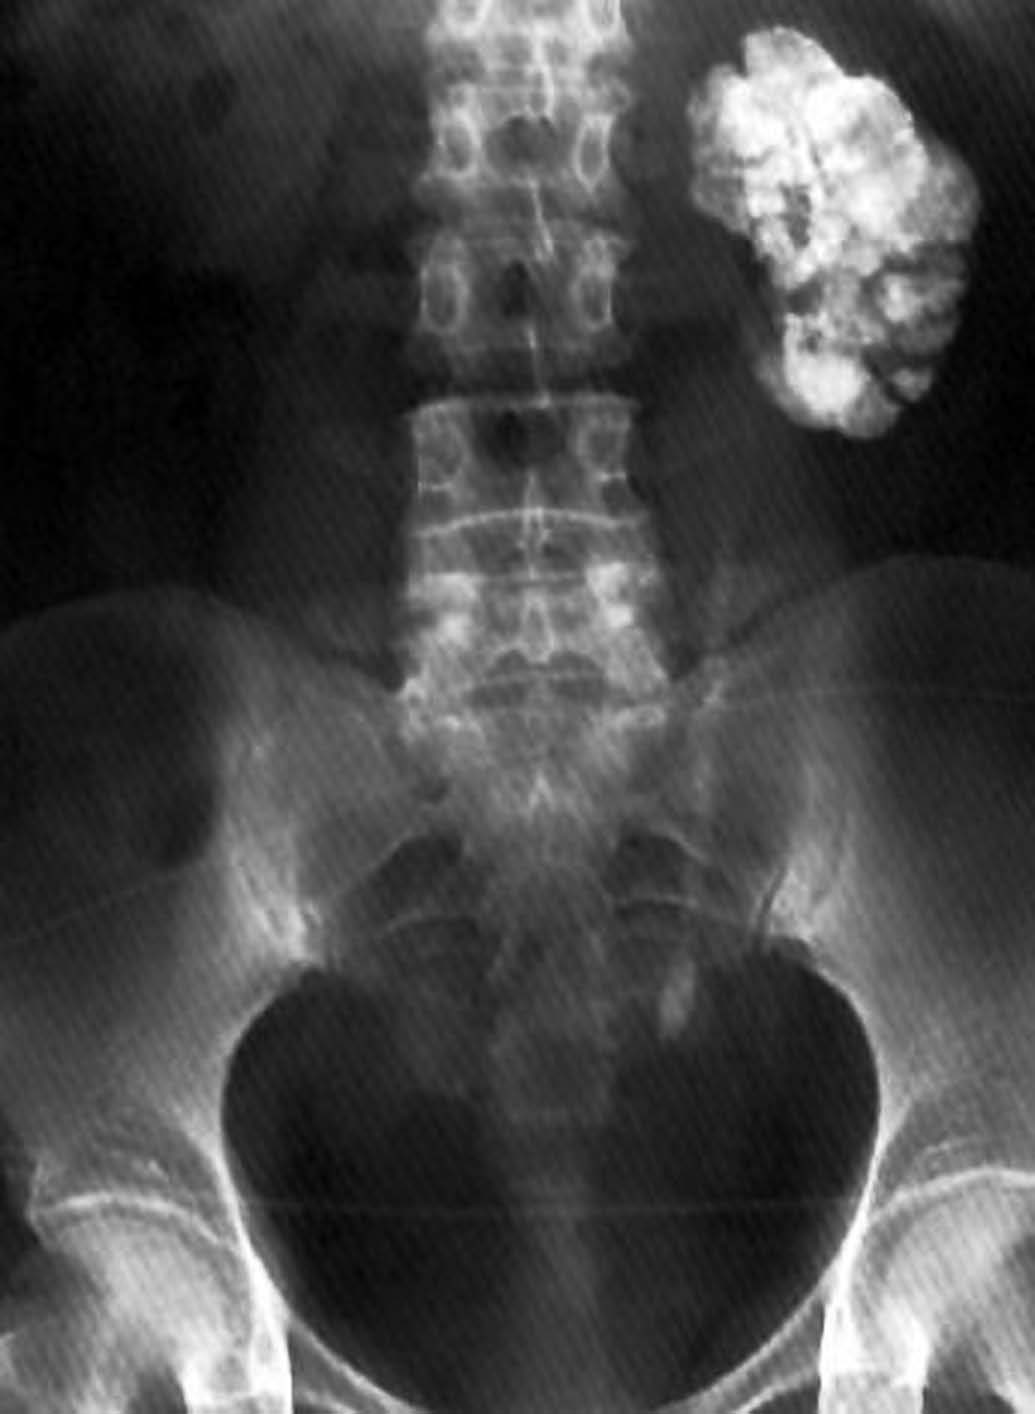
\includegraphics{./images/Image00376.jpg}
    \captionsetup{justification=centering}
    \caption{KUB平片}
    \label{fig6-4-4}
\end{figure}

\textbf{【病史摘要】}
女性,30岁。有肾结核病史5年,近来左腰部酸痛加重。

\textbf{【X线表现】}  左肾大量不规则钙化,左侧输尿管中上段钙化。

\textbf{【X线诊断】}  左肾左输尿管结核晚期,左肾自截。

\textbf{【评  述】}
病变波及整个肾脏,全肾广泛破坏,破坏的囊腔内充满干酪坏死物质,然后大量钙质沉积,并形成肾大部或全部钙化且肾功能完全丧失。

\subsection{输尿管结核}

\begin{figure}[!htbp]
    \centering
    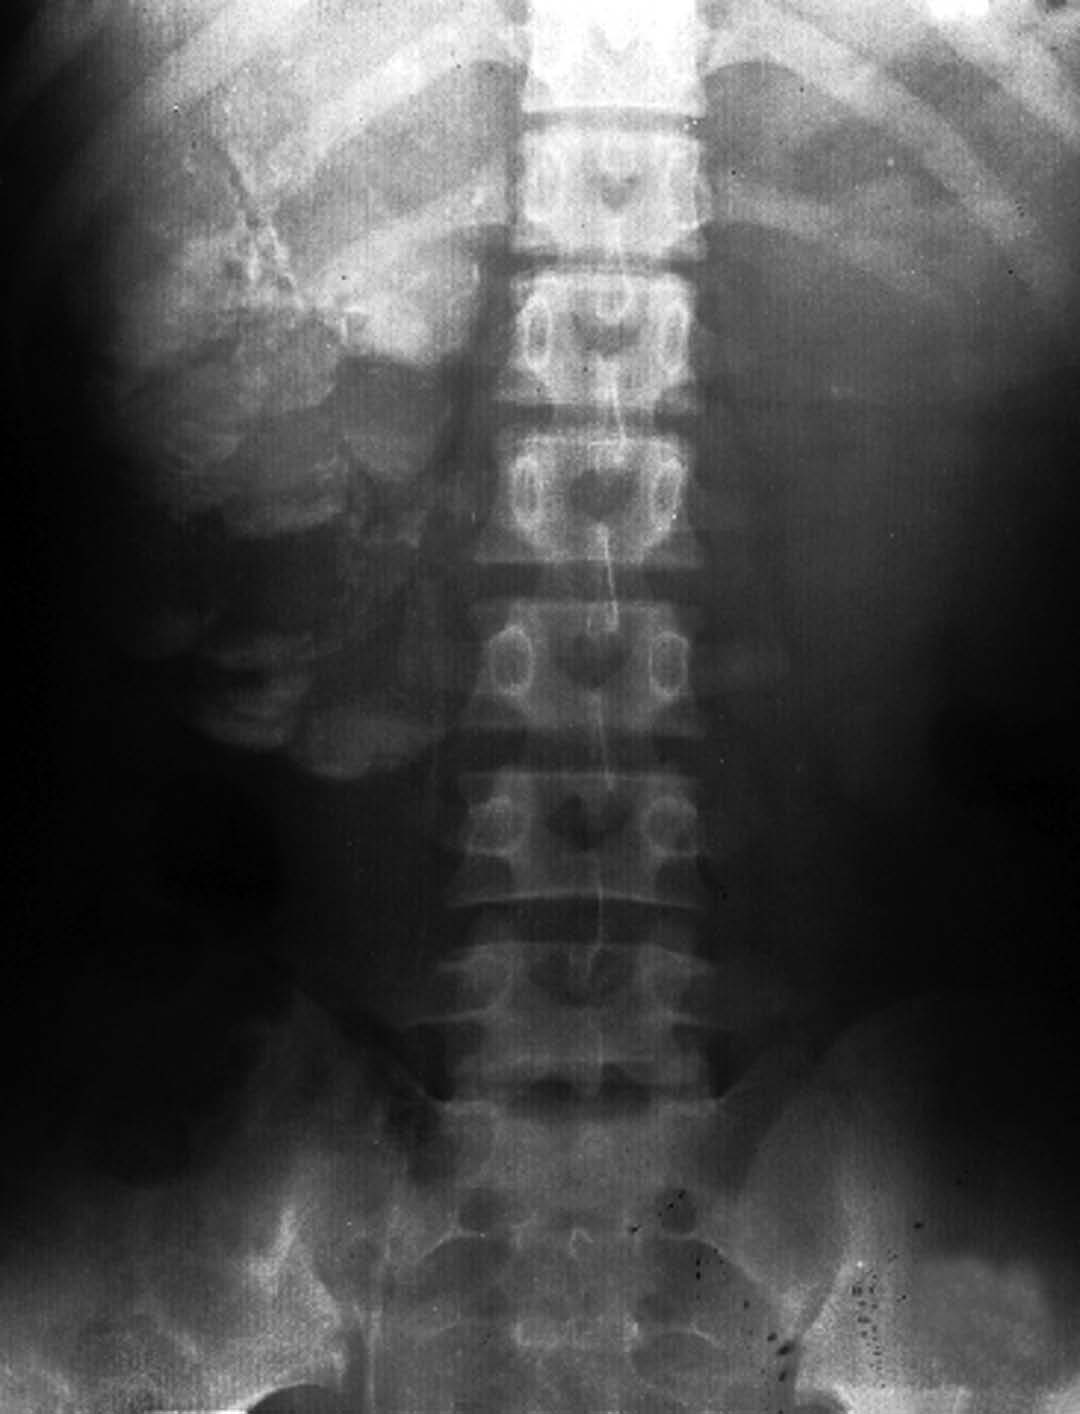
\includegraphics{./images/Image00377.jpg}
    \captionsetup{justification=centering}
    \caption{KUB平片}
    \label{fig6-4-5}
\end{figure}

\textbf{【病史摘要】}
女性,32岁。肾结核病史3年,近来右腰部酸胀明显加重。

\textbf{【X线表现】}  腹部平片示:右肾不规则钙化,右输尿管钙化。

\textbf{【X线诊断】}  右肾及右输尿管结核后期。

\textbf{【评  述】}
输尿管结核由肾结核蔓延而来,结核致输尿管改变主要为粘膜溃疡和管壁纤维化形成狭窄,狭窄与扩张相间存在,影响尿液的引流。造影片上可见串珠样改变。晚期可见管壁的条状钙化。

\subsection{慢性肾盂肾炎}

\begin{figure}
    \centering
    \subfloat[KUB平片]{
        \begin{minipage}[b]{0.48\textwidth}
            \centering
            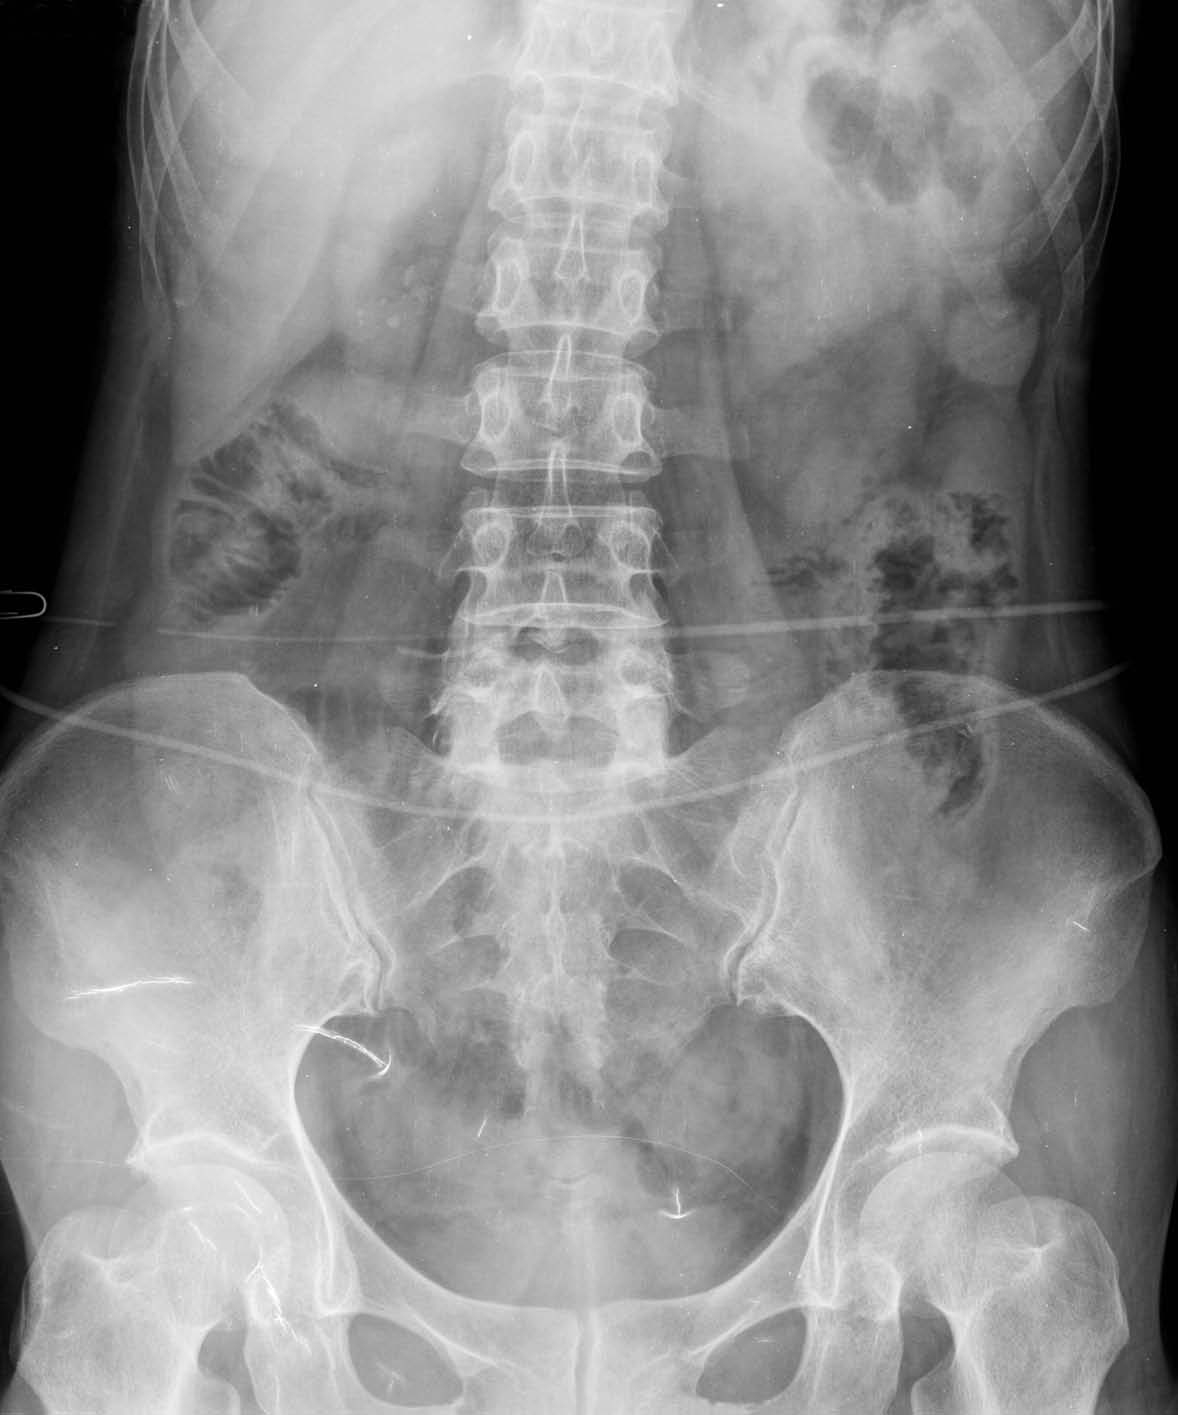
\includegraphics{./images/Image00378.jpg}
        \end{minipage}}
    \subfloat[IVP16分钟平片]{
        \begin{minipage}[b]{0.48\textwidth}
            \centering
            \includegraphics{./images/Image00379.jpg}
        \end{minipage}}\\
    \subfloat[IVP32分钟平片]{
        \begin{minipage}[b]{0.48\textwidth}
            \centering
            \includegraphics{./images/Image00380.jpg}
        \end{minipage}}\\
    \caption{}
    \label{fig6-4-6}
\end{figure}

\textbf{【病史摘要】}
女性,58岁。右腰痛数年,尿白细胞增高,镜下血尿(++)。

\textbf{【X线表现】}
右肾体积缩小,右肾实质见不规则高密度影,右肾显影延迟。

\textbf{【X线诊断】}  结合病史,考虑右侧肾盂肾炎。

\textbf{【评  述】}
肾盂肾炎好发于女性。多为逆行感染所致,亦可因先天性发育异常或结石引起阻塞而继发感染。此外,血行和淋巴的传染途径亦很重要。常见的致病菌为大肠杆菌。病变多为双侧感染,因纤维组织增生和瘢痕收缩,使得肾脏轮廓呈分叶状。肾盂、肾盏变形僵硬、扭曲,边缘变钝而平有扩大积水现象。肾萎缩可致皮质变薄。肾功能受损,可致肾盂、肾盏的显影延迟和密度减低。本病变需与先天性小肾和肾血管性狭窄引起的肾萎缩鉴别。本病确诊需结合实验室检查。静脉肾盂造影可观察肾功能情况及病变程度。

\subsection{输尿管炎}

\begin{figure}
    \centering
    \subfloat[KUB平片]{
        \begin{minipage}[b]{0.48\textwidth}
            \centering
            \includegraphics{./images/Image00381.jpg}
        \end{minipage}}
    \subfloat[IVP32分钟平片]{
        \begin{minipage}[b]{0.48\textwidth}
            \centering
            \includegraphics{./images/Image00382.jpg}
        \end{minipage}}\\
    \caption{}
    \label{fig6-4-7}
\end{figure}

\textbf{【病史摘要】}  男性,60岁。腰痛,尿蛋白增高,镜下血尿(++)。

\textbf{【X线表现】}
尿路造影示:左侧输尿管略僵硬,壁略毛糙,管腔不均匀性狭窄伴扩张。

\textbf{【X线诊断】}  左侧输尿管炎。

\textbf{【评  述】}
输尿管炎为输尿管的炎性改变,常继发于肾盂肾炎、膀胱炎等,部分患者因尿路器械检查、尿路结石而发生,由于粘膜和肌层病变表现为输尿管壁的变硬、僵直、变薄、扩张与狭窄相间。本病需与结核性输尿管炎及输尿管乳头状瘤鉴别诊断。前者有肾结核病史,后者主要表现为静脉肾盂造影上输尿管局限性的充盈缺损。

\section{泌尿系肿瘤}

\subsection{肾细胞癌}

\begin{figure}
    \centering
    \subfloat[KUB平片]{
        \begin{minipage}[b]{0.48\textwidth}
            \centering
            \includegraphics{./images/Image00383.jpg}
        \end{minipage}}
    \subfloat[IVP16分钟片]{
        \begin{minipage}[b]{0.48\textwidth}
            \centering
            \includegraphics{./images/Image00384.jpg}
        \end{minipage}}\\
    \subfloat[IVP32分钟片]{
        \begin{minipage}[b]{0.48\textwidth}
            \centering
            \includegraphics{./images/Image00385.jpg}
        \end{minipage}}\\
    \caption{}
    \label{fig6-5-1}
\end{figure}

\textbf{【病史摘要】}  男性,58岁。体检时B超发现右肾占位。

\textbf{【X线表现】}
右肾下极膨隆,右肾体积明显增大,尿路造影示右侧肾盂、肾盏向上推移。

\textbf{【X线诊断】}  右肾癌。

\textbf{【评  述】}
肾细胞癌为肾脏最常见的恶性肿瘤,来源于肾小管上皮,发生于肾实质内。肿瘤大小不一,大多伴有出血坏死、纤维化斑块,中心坏死区形成囊肿。肿瘤内可见钙化。肾癌易侵犯肾筋膜及肾包膜以及周围结构,并易形成肾静脉及下腔静脉癌栓。晚期可血行转移到肺、脑、骨、肝、肾上腺等全身各个脏器。X线平片上主要观察肾脏轮廓的改变及有无钙化灶。静脉肾盂造影上,当肿瘤生长到一定程度,可对肾盂、肾盏产生压迫及破坏。使肾盂、肾盏牵拉变长、变形、变细、扭曲,甚至数个小盏破坏、闭锁或分离,形成蜘蛛足样征。较小的肾癌在静脉肾盂造影上无明显表现,与肾囊肿也较难鉴别。需行CT或MRI检查以明确诊断。

\subsection{肾胚胎瘤}

\begin{figure}[!htbp]
    \centering
    \includegraphics{./images/Image00386.jpg}
    \captionsetup{justification=centering}
    \caption{IVP平片}
    \label{fig6-5-2}
\end{figure}

\textbf{【病史摘要】}
1岁幼儿。偶尔发现腹部膨隆,体检时发现腹部巨大肿块。

\textbf{【X线表现】}
IVP示:右肾未显影,见巨大软组织肿块影,左肾盂、肾盏显影可。

\textbf{【X线诊断】}  右肾胚胎瘤。

\textbf{【评  述】}
肾胚胎瘤又称肾母细胞瘤或Wilms瘤,1899年Wilms对该病做了详细阐述。为小儿最常见的肿瘤,占小儿恶性肿瘤的10%\textbf{~}
24%。发病年龄自出生后12小时至83岁,但以6个月至3岁组最常见。90%的病例小于7岁。双侧发病占1%\textbf{~}
10%。临床表现主要的症状为腹部肿块,常为家长偶尔发现。X线平片上为患侧肾影明显增大,或肿块影与肾影融合呈巨大软组织包块。患侧腰大肌影可模糊,肿块内偶见钙化,呈弧线状或粗颗粒状,常位于肿瘤的边缘。静脉肾盂造影可见肾盂、肾盏发生明显的压迫、旋转、移位、扩张、变形、拉长、分离和破坏等异常。部分病例可由于肿瘤肾组织的大量破坏及肾静脉栓塞使病变肾脏不显影。本病需与后腹膜肿瘤鉴别诊断,如肾癌、神经母细胞瘤、腹膜后畸胎瘤等病变鉴别。CT及MRI检查可进一步明确诊断。

\subsection{肾盂癌}

\begin{figure}
    \centering
    \subfloat[KUB平片]{
        \begin{minipage}[b]{0.48\textwidth}
            \centering
            \includegraphics{./images/Image00387.jpg}
        \end{minipage}}
    \subfloat[IVP16分钟平片]{
        \begin{minipage}[b]{0.48\textwidth}
            \centering
            \includegraphics{./images/Image00388.jpg}
        \end{minipage}}\\
    \subfloat[IVP32分钟平片]{
        \begin{minipage}[b]{0.48\textwidth}
            \centering
            \includegraphics{./images/Image00389.jpg}
        \end{minipage}}\\
    \caption{}
    \label{fig6-5-3}
\end{figure}

\textbf{【病史摘要】}  男性,60岁。肉眼血尿,伴左侧腰部胀痛。

\textbf{【X线表现】}
KUB平片示:未见明显异常,尿路造影示左侧肾盂扩张,其内见不规则充盈缺损,左侧肾盏杯口消失,左输尿管未显影。膀胱显影好,边界光整,未见明显充盈缺损。

\textbf{【X线诊断】}  左侧肾盂癌。

\textbf{【评  述】}
肾盂癌来源于肾盂上皮细胞,好发于40岁以上的成年人,以50\textbf{~}
70岁以上更多见,男女比例为2\textbf{~}
4∶1。大多肿瘤生长缓慢,主要的临床症状为血尿。病理上,肾盂肿瘤85%\textbf{~}
95%为移行细胞癌,大约10%为鳞状细胞癌,腺癌非常罕见。肾盂乳头状瘤是指细胞分化程度较好,组织结构类似良性病变的肿瘤,极易恶变,应视为早期恶性病变。X线平片常无异常发现。静脉肾盂造影可见肾盂或肾盏内出现固定不变的充盈缺损,其大小、形状及数目随肿瘤生长的情况而定。当发现肾盂内有充盈缺损时,应仔细观察输尿管及膀胱是否有充盈缺损存在,因肾盂肿瘤可移植到输尿管及膀胱。CTU可显示与静脉肾盂造影类似的图像,同时可观察病灶及与周围组织的关系。对静脉肾盂造影不显影病变可行MRU检查。造成肾盂占位的病变较多,需与肾盂癌鉴别。①黄色肉芽肿性肾盂肾炎。本病为慢性肾盂肾炎,由于肾盂与输尿管连接部梗阻,反复感染炎症引起,可引起肾盂、肾盏扩大,其内密度较高,与肾盂癌相似。大约80%合并肾盂或肾盏内结石,CT扫描时增强后肾盂内无强化。②肾盂血肿。临床有血尿,静脉肾盂造影上肾盂内见充盈缺损。应做CT扫描,血肿密度较高,增强后无强化。③肾癌。肾癌侵犯肾盂时,与肾盂癌相似,CT扫描可作鉴别,一般肾癌的血供丰富,肿瘤常引起肾脏轮廓改变,肿瘤内较多出血坏死。④肾盂旁囊肿。CT上囊内为水样密度,增强后无强化。⑤多房囊性肾瘤。可发生在肾盂内,病变由多数小的囊腔构成,CT扫描可为软组织密度,增强后有不均匀强化。较难鉴别时需结合其他影像学检查方法。

\subsection{输尿管癌}

\begin{figure}[!htbp]
    \centering
    \includegraphics{./images/Image00390.jpg}
    \captionsetup{justification=centering}
    \caption{IVP平片}
    \label{fig6-5-4}
\end{figure}

\textbf{【病史摘要】}  男性,60岁。腰痛,肉眼血尿。

\textbf{【X线表现】}
左侧输尿管多发充盈缺损,边缘略毛糙,管壁僵硬,管腔粗细不均。

\textbf{【X线诊断】}  左侧输尿管癌

\textbf{【评  述】}
输尿管移行细胞癌少见,占上尿路肿瘤的1%\textbf{~}
3%。肿瘤好发年龄为50\textbf{~}
70岁,男女比例为3∶1。临床表现主要为血尿,多为无痛性全程或终末血尿。大量的血凝块阻塞输尿管可引起肾绞痛。输尿管肿瘤多发生于左侧,更常见的在下1/3段,病变可单发或多发,也可双侧发生,病变可由肾盂、膀胱肿瘤种植或蔓延引起。输尿管肿瘤大部分为恶性,90%以上为移行细胞癌,鳞癌、腺癌相对少见。

常规尿路造影为输尿管肿瘤检查的重要方法。其优点是可观察肾脏、输尿管及膀胱的情况。X线平片,可无阳性发现,如肾脏积水严重,可见肾影增大。静脉肾盂造影可见输尿管腔内圆形或分叶状的充盈缺损。由于输尿管癌形成的梗阻为慢性梗阻,梗阻远端输尿管扩张,扩张的输尿管与充盈缺损形成高脚酒杯征。该征象具有一定特征性。本病需与阴性结石及血凝块形成的梗阻鉴别,由于结石与血凝块为急性梗阻,梗阻远端输尿管形成痉挛收缩,没有输尿管肿瘤形成的高脚酒杯征。

\subsection{膀胱癌}

\begin{figure}
    \centering
    \subfloat[KUB平片]{
        \begin{minipage}[b]{0.48\textwidth}
            \centering
            \includegraphics{./images/Image00391.jpg}
        \end{minipage}}
    \subfloat[IVP32分钟平片]{
        \begin{minipage}[b]{0.48\textwidth}
            \centering
            \includegraphics{./images/Image00392.jpg}
        \end{minipage}}\\
    \caption{}
    \label{fig6-5-5}
\end{figure}

\textbf{【病史摘要】}  男性,65岁。肉眼血尿1周。

\textbf{【X线表现】}
尿路造影示:膀胱左输尿管入口处见不规则小充盈缺损,边缘毛糙。

\textbf{【X线诊断】}  膀胱癌。

\textbf{【评  述】}
膀胱肿瘤为泌尿系统比较常见的肿瘤,以恶性肿瘤为多见。男性多于女性,为2\textbf{~}
4∶1。膀胱肿瘤以上皮来源肿瘤最常见,其中以乳头状瘤、乳头状癌的发病率最高。膀胱肿瘤常为单发,亦可多发。绝大多数肿瘤位于膀胱三角区和两侧壁。造影检查为膀胱癌的重要检查方法。主要征象为局部充盈缺损,肿瘤轮廓不规则。肿瘤可引起输尿管开口阻塞。肿瘤较小者,可能无阳性发现,膀胱镜检查可确诊。膀胱癌应与下列疾病鉴别:①膀胱血块。形态不规则,变换体位,血块位置可变。CT扫描密度较高,无强化。②腺性膀胱炎。乳头状瘤型腺性膀胱炎的影像学表现与膀胱肿瘤极为相似,确诊靠病理检查。③前列腺增生。前列腺增生多见于老年人,膀胱底部有边缘光滑的半球形压迹。

\section{肾囊肿性病变}

\subsection{多囊肾}

\begin{figure}[!htbp]
    \centering
    \includegraphics{./images/Image00393.jpg}
    \captionsetup{justification=centering}
    \caption{IVP平片}
    \label{fig6-6-1}
\end{figure}

\textbf{【病史摘要】}  男性,54岁。右腰痛,加重1周。

\textbf{【X线表现】}  右侧肾盂、肾盏伸长、变细,并显示多处弧形压迹。

\textbf{【X线诊断】}  右侧多囊肾。

\textbf{【评  述】}
多囊肾为先天性囊肿,为常染色体显性遗传性疾病。95%\textbf{~}
98%发生于两侧肾脏。病理上,两侧肾脏皮质及髓质满布大小不等的囊肿。临床上幼年时很少出现症状,一般30岁以后出现症状,表现为肾脏增大、局部不适、血尿、蛋白尿、高血压等。晚期出现慢性肾衰竭。静脉肾盂造影表现为两侧肾影增大,边缘可呈波浪形,两侧的肾盂、肾盏不同程度地受压、变形和分离。肾盏边缘出现半月形压迹、颈部伸长,有时可呈一种特殊的蜘蛛足状,肾盂、肾盏的本身和大小肾盏都伸直、增长和狭窄。肾功能常有不同程度的受损。与肾癌鉴别:本病为两侧性,累及全肾,不造成肾盂、肾盏的侵蚀、破坏,必要时行CT及MR鉴别。

\subsection{肾囊肿}

\begin{figure}
    \centering
    \subfloat[KUB平片]{
        \begin{minipage}[b]{0.48\textwidth}
            \centering
            \includegraphics{./images/Image00394.jpg}
        \end{minipage}}
    \subfloat[IVP32分钟平片]{
        \begin{minipage}[b]{0.48\textwidth}
            \centering
            \includegraphics{./images/Image00395.jpg}
        \end{minipage}}\\
    \caption{}
    \label{fig6-6-2}
\end{figure}

\textbf{【病史摘要】}  女性,62岁。B超发现左肾囊肿1个月。

\textbf{【X线表现】}
KUB示:左肾下极膨大明显,边界清晰。尿路造影示:左侧肾盂、肾盏受压向上推移,肾盏杯口锐利。双侧输尿管通畅。

\textbf{【X线诊断】}  左肾囊肿。

\textbf{【评  述】}
单纯性肾囊肿最为常见,主要发生于成年人,随着年龄增加,50岁以上约有一半人至少肾上有一个囊肿。肾囊肿的病理机制不甚明了,囊肿多见于肾皮质。囊壁薄内衬以单层扁平上皮细胞。平片上较大的囊肿可见轮廓的改变,边缘较光整。静脉肾盂造影见肾盏受压、伸长、移位和新月状变形,边缘光滑锐利,通常囊肿不显影。囊肿部位密度较浅,有时与肾癌较难鉴别,CT或MR检查可与之鉴别。

\subsection{肾盏憩室}

\begin{figure}
    \centering
    \subfloat[KUB平片]{
        \begin{minipage}[b]{0.48\textwidth}
            \centering
            \includegraphics{./images/Image00396.jpg}
        \end{minipage}}
    \subfloat[IVP16分钟平片]{
        \begin{minipage}[b]{0.48\textwidth}
            \centering
            \includegraphics{./images/Image00397.jpg}
        \end{minipage}}\\
    \subfloat[IVP32分钟平片]{
        \begin{minipage}[b]{0.48\textwidth}
            \centering
            \includegraphics{./images/Image00398.jpg}
        \end{minipage}}\\
    \caption{}
    \label{fig6-6-3}
\end{figure}

\textbf{【病史摘要】}  男性,30岁。腰痛,镜下血尿(+)。

\textbf{【X线表现】}
KUB未见明显异常,尿路造影示右侧肾上盏上方见囊性造影剂充填区,边界光整。

\textbf{【X线诊断】}  右肾上盏憩室。

\textbf{【评  述】}
有人认为肾盏憩室就是肾盂源性囊肿,但其病理基础不一样,不是先天性的。该病的病理机制是由于肾盏颈部的肌肉功能紊乱,肌肉发生痉挛,然后因缺血而产生纤维化,进而发生狭窄阻塞,在其远端部分的肾盏就可扩大,并分离而成为憩室。狭窄段就成为原来的肾盏与新形成的憩室之间相通的细管。平片上常无异常发现。静脉肾盂造影憩室可显影,大的憩室内残留的尿液稀释造影剂使得开始显影较淡,延迟后显影逐渐增高,此时诊断可确诊。

\subsection{肾盂源性囊肿}

\begin{figure}
    \centering
    \subfloat[KUB平片]{
        \begin{minipage}[b]{0.48\textwidth}
            \centering
            \includegraphics{./images/Image00399.jpg}
        \end{minipage}}
    \subfloat[IVP 32分钟平片]{
        \begin{minipage}[b]{0.48\textwidth}
            \centering
            \includegraphics{./images/Image00400.jpg}
        \end{minipage}}\\
    \caption{}
    \label{fig6-6-4}
\end{figure}

\textbf{【病史摘要】}  女性,41岁。体检时B超示左肾局限性积水。

\textbf{【X线表现】}
KUB未见明显异常,尿路造影示左肾下盏基底部见向外突出囊性略高密度影。

\textbf{【X线诊断】}  左肾肾盂源性囊肿。

\textbf{【评  述】}
肾盂源性囊肿大小为2~4cm,大多位于肾髓质部,且在大肾盏或肾盂旁,与囊肿之间常有一细管相通。但不一定能显示。静脉肾盂造影见肾功能正常,囊肿较大时在肾盂、肾盏上造成压迹。囊肿通常不显影。本病需与肾结核瘤鉴别,后者常见肿块内有钙化且造影时不显影。

\subsection{海绵肾}

\begin{figure}
    \centering
    \subfloat[KUB平片]{
        \begin{minipage}[b]{0.3\textwidth}
            \centering
            \includegraphics[height=.2\textheight]{./images/Image00401.jpg}
        \end{minipage}}
    \subfloat[IVP 16分钟平片]{
        \begin{minipage}[b]{0.38\textwidth}
            \centering
            \includegraphics[height=.2\textheight]{./images/Image00402.jpg}
        \end{minipage}}
    \subfloat[IVP 32分钟平片]{
        \begin{minipage}[b]{0.3\textwidth}
            \centering
            \includegraphics[height=.2\textheight]{./images/Image00403.jpg}
        \end{minipage}}\\
    \caption{}
    \label{fig6-6-5}
\end{figure}

\textbf{【病史摘要】}
女性,55岁。腰部酸痛,加重数月,镜下血尿(+++)。

\textbf{【X线表现】}
KUB示:双侧肾脏多发弥漫性微小钙化灶。尿路造影示:双侧肾盏扩张积水,结石位于肾盏周围。

\textbf{【X线诊断】}  双侧髓质海绵肾。

\textbf{【评  述】}
本病是一种先天性非特异性肾集合小管的扩大。70%系双肾患病,每侧肾脏有一个至数个乳头受累。在平片上可见双肾广泛存在微小结石。静脉肾盂造影是很重要的检查方法,可以显示造影剂潴留在扩大的肾小管、乳头管及小囊肿,还可确定结石特殊的位置。典型病例根据钙化的形态与分布可以明确诊断。

\section{其他}

\subsection{肾下垂}

\begin{figure}
    \centering
    \subfloat[KUB平片]{
        \begin{minipage}[b]{0.3\textwidth}
            \centering
            \includegraphics[height=.25\textheight]{./images/Image00404.jpg}
        \end{minipage}}
    \subfloat[IVP 16分钟平片]{
        \begin{minipage}[b]{0.38\textwidth}
            \centering
            \includegraphics[height=.25\textheight]{./images/Image00405.jpg}
        \end{minipage}}
    \subfloat[IVP 32分钟平片]{
        \begin{minipage}[b]{0.3\textwidth}
            \centering
            \includegraphics[height=.25\textheight]{./images/Image00406.jpg}
        \end{minipage}}\\
    \caption{}
    \label{fig6-7-1}
\end{figure}

\textbf{【病史摘要】}  女性,50岁。腰酸,加重1周,镜下血尿(+)。

\textbf{【X线表现】}
双侧肾脏位置下移,肾门位于L2/3椎间隙水平,余未见明显异常。

\textbf{【X线诊断】}  双侧肾下垂。

\textbf{【评  述】}
肾的位置自卧位变换到立位时可下降两个椎体以上的距离。患者的年龄一般较大,且伴有其他内脏下垂。由于肾脏的移动度较大,引起排空延迟,容易产生肾盂、肾盏积水而并发感染。X线检查主要依靠静脉肾盂造影,肾脏显影时,分别摄卧位及立位片,此时下垂的一侧肾脏常可下降达两个以上椎体的距离。鉴别诊断主要与先天性游走肾和异位肾鉴别。先天性游走肾的输尿管特别长,且肾脏活动的范围亦不受限制。而异位肾位于盆腔内时输尿管特别短,且肾脏的血供多来自髂动脉。

\subsection{神经源性膀胱}

\begin{figure}
    \centering
    \subfloat[KUB平片]{
        \begin{minipage}[b]{0.48\textwidth}
            \centering
            \includegraphics[height=.22\textheight]{./images/Image00407.jpg}
        \end{minipage}}
    \subfloat[IVP 32分钟平片]{
        \begin{minipage}[b]{0.48\textwidth}
            \centering
            \includegraphics[height=.22\textheight]{./images/Image00408.jpg}
        \end{minipage}}\\
    \caption{}
    \label{fig6-7-2}
\end{figure}

\textbf{【病史摘要】}  男性,56岁。肉眼血尿10余天。

\textbf{【X线表现】}
KUB示:膀胱体积增大,边界欠光整。尿路造影示:膀胱显影密度不均。

\textbf{【X线诊断】}  神经源性膀胱。

\textbf{【评  述】}
由于支配膀胱的外周神经或中枢神经发生障碍时均可发生排尿障碍,这种神经功能性排尿障碍导致的膀胱病变就是神经源性膀胱。高级中枢损伤:由于膀胱张力持续升高,膀胱造影表现为膀胱壁增厚,膀胱小梁或憩室形成,憩室不大,数目较多,可有结石,由于膀胱括约肌痉挛,膀胱内缘可呈高低不平小波浪状,膀胱体积常增大,典型呈宝塔形。低级中枢损伤:膀胱张力低,膀胱体积明显增大,膀胱表面光滑。鉴别诊断:慢性膀胱炎伴下尿路梗阻,影像学表现与神经源性膀胱较难鉴别,需结合病史,有无神经损伤的相应表现。

\subsection{尿道及膀胱异物}

\begin{figure}[!htbp]
    \centering
    \includegraphics{./images/Image00409.jpg}
    \captionsetup{justification=centering}
    \caption{膀胱区平片}
    \label{fig6-7-3}
\end{figure}

\textbf{【病史摘要】}  男性,11岁。铅笔芯断入尿道5小时。

\textbf{【X线表现】}  尿道海绵体部见点状高密度影。

\textbf{【X线诊断】}  尿道异物。

\textbf{【评  述】}
尿道及膀胱异物,最多为经尿道外口插入。少数为外伤或前列腺手术时遗留于尿道内。男性多见。异物种类较多,金属异物平片可见,异物在膀胱中可以以异物为中心形成结石,但较少见。在平片无法显示的异物,CT较易诊断。

\section{肾上腺疾病}

\subsection{肾上腺嗜铬细胞瘤}

\begin{figure}[!htbp]
    \centering
    \includegraphics{./images/Image00410.jpg}
    \captionsetup{justification=centering}
    \caption{腹膜后充气造影}
    \label{fig6-8-1}
\end{figure}

\textbf{【病史摘要】}  男性,25岁。高血压,血糖增高,消瘦。

\textbf{【X线表现】}
腹膜后充气造影示:右侧肾上腺体积明显增大,呈肿块样改变。

\textbf{【X线诊断】}  右侧肾上腺嗜铬细胞瘤。

\textbf{【评  述】}
嗜铬细胞瘤是一种产生儿茶酚胺的肿瘤,占初诊高血压患者的0.5%,肿瘤的诊断具有重要的临床意义,切除肿瘤可以治愈高血压。嗜铬细胞瘤好发于青壮年。肿瘤90%发生于肾上腺,10%位于肾上腺之外,10%为恶性,10%为多发肿瘤,因此称为10%肿瘤。嗜铬细胞瘤的典型临床症状为阵发性高血压、头痛、心悸、多汗,发作数分钟后症状缓解。原发性肾上腺占位性病灶常见还有肾上腺腺瘤。仅靠X线无法区分肿瘤类型,较小的肿瘤不易发现。必须行CT或MR检查,对诊断及鉴别诊断具有较重要的作用。

\protect\hypertarget{text00012.html}{}{}

